\chapter{\acrshort{ux} \& \acrshort{ui} design} \label{chapter4}

Because our survey indicated that we need to pay special attention to designing the interface of our application (see section \ref{3:appearance}), we decided to take an iterative approach to defining the \acrlong{ux} (\acrshort{ux}), and, by extension, sketching the \acrlong{ui} (\acrshort{ui}).

\section{Requirements} \label{4:requirements}

The proposed functionalities of our application are listed in section \ref{1:functionalities}. We will aim to reach our goals, as described in section \ref{1:goals}.

We will be designing a collaborative application (a decision motivated in section \ref{2:mix_and_match}) with a moderation system based on permission levels, described in this chapter in section \ref{4:permissions}.

Based on the results of our survey (section \ref{3:appearance}), our design language of choice will be neither Google's Material Design\cite{google2020material}, nor Apple's Human Interface Guidelines\cite{apple2020human}, but rather what we consider to be a healthy mix of both. This design aims to be pleasant for both Android and iOS users, as is required of a cross-platform application which aims to have a consistent design on all platforms. A good example of another such application is \textit{Reddit} (available on both the App Store\footnote{https://apps.apple.com/us/app/reddit/id1064216828} and Google Play\footnote{https://play.google.com/store/apps/details?id=com.reddit.frontpage} with a very similar design that only slightly differs in the web version\footnote{http://reddit.com/}). However, since it sports a platform-agnostic design, independent developers have come up with separate applications for viewing \textit{Reddit} content on Android and iOS devices, which claim to have a more "native" look for the more nitpicky users. A visual comparison between these applications can be seen in appendix \ref{a:native_cross}.

\section{Paper prototyping} \label{4:paper}

\subsection{Initial concept} \label{4:paper_concept}

We kick-started the design process by making a rough sketch of what we imagined the app to look like, on paper, with the features we had in mind in the beginning. We used the \textit{School Assistant} app (see section \ref{2:generic_apps}) as the main inspiration for this first design.

\begin{figure}[ht]
    \centering
         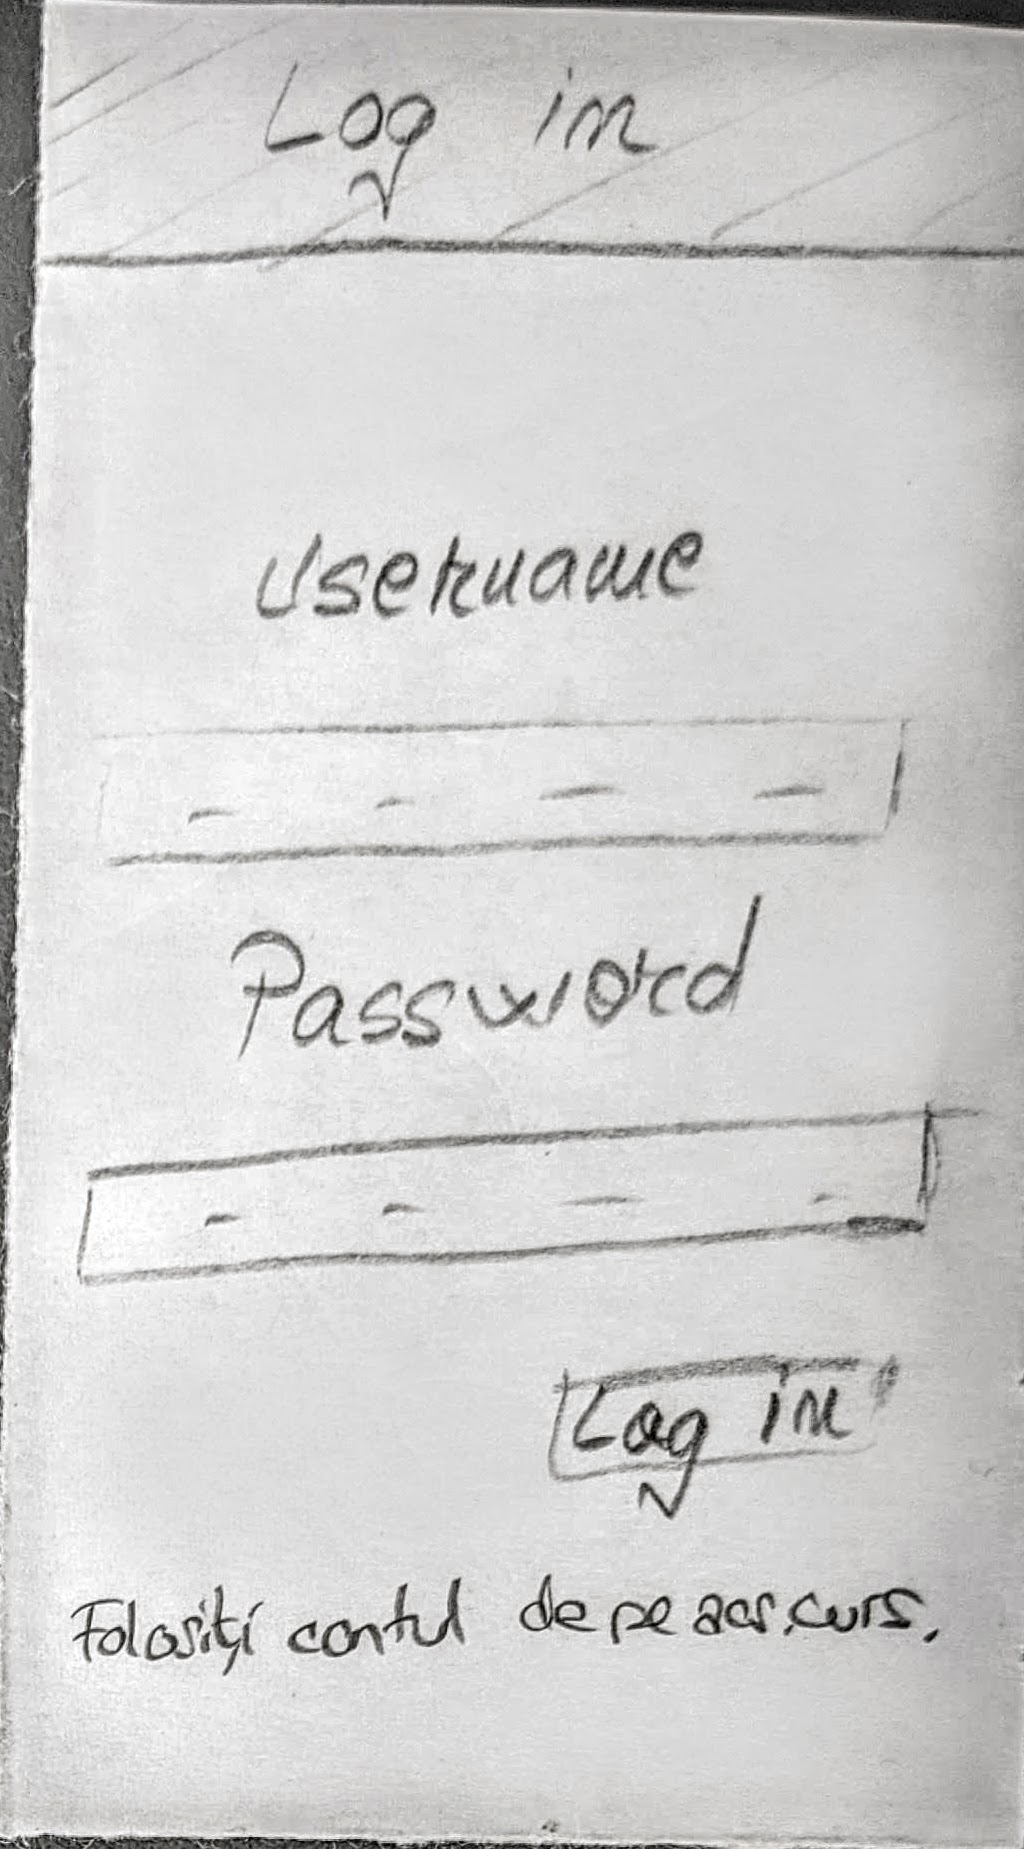
\includegraphics[height=0.279\textheight]{figures/app/paper/login.jpg}
         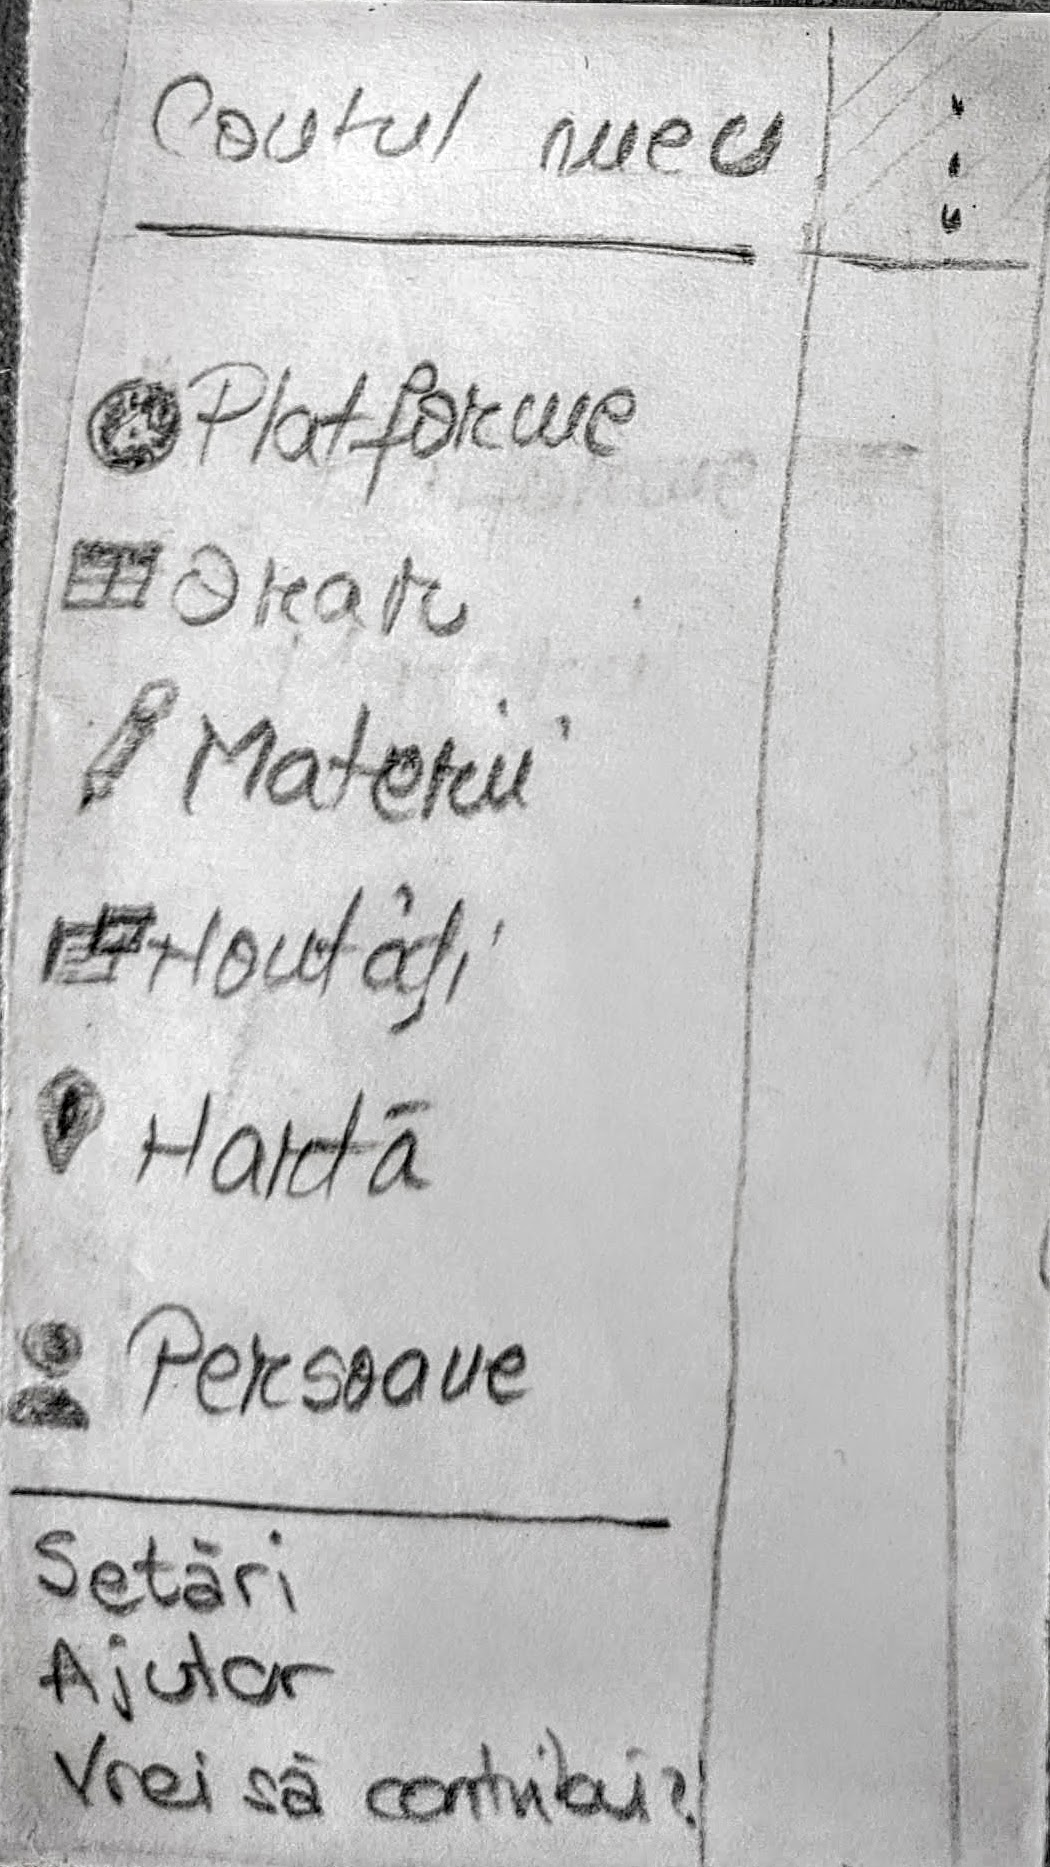
\includegraphics[height=0.279\textheight]{figures/app/paper/drawer.jpg}
         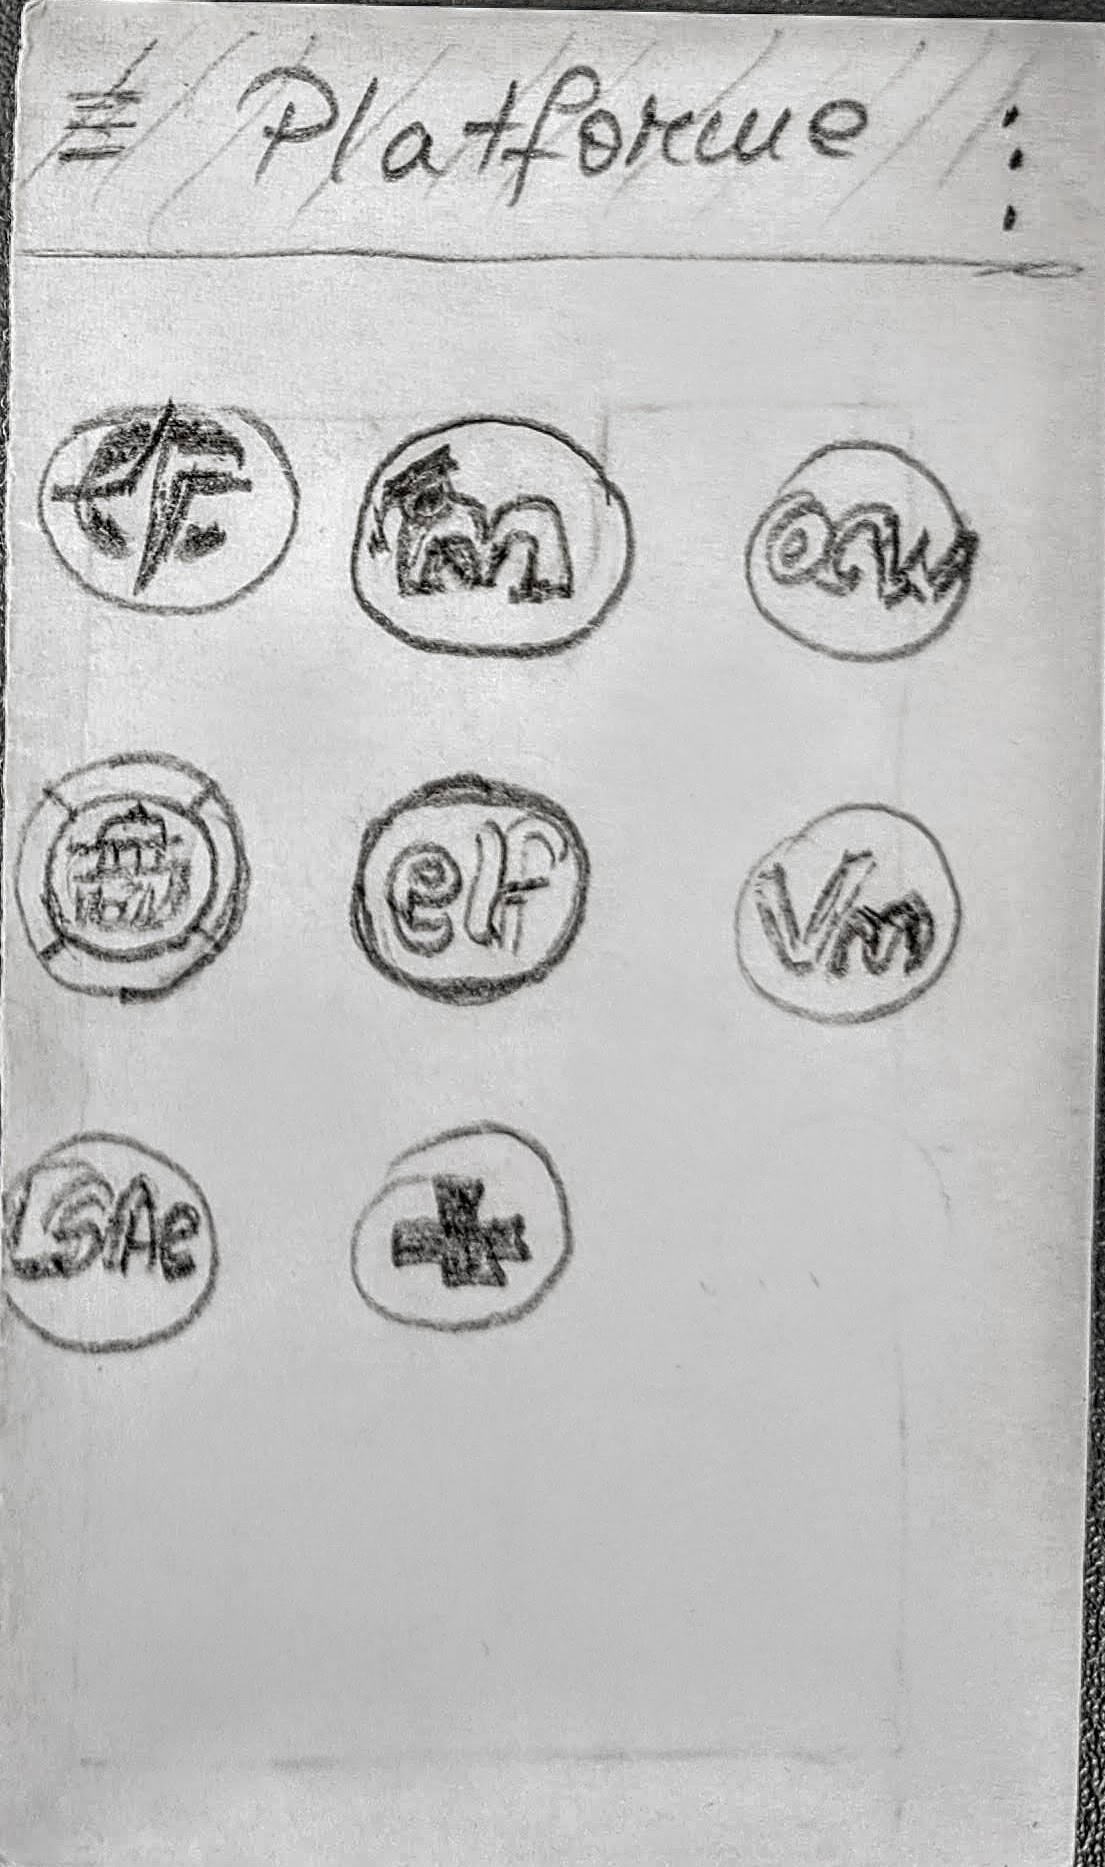
\includegraphics[height=0.279\textheight]{figures/app/paper/platforms.jpg}
         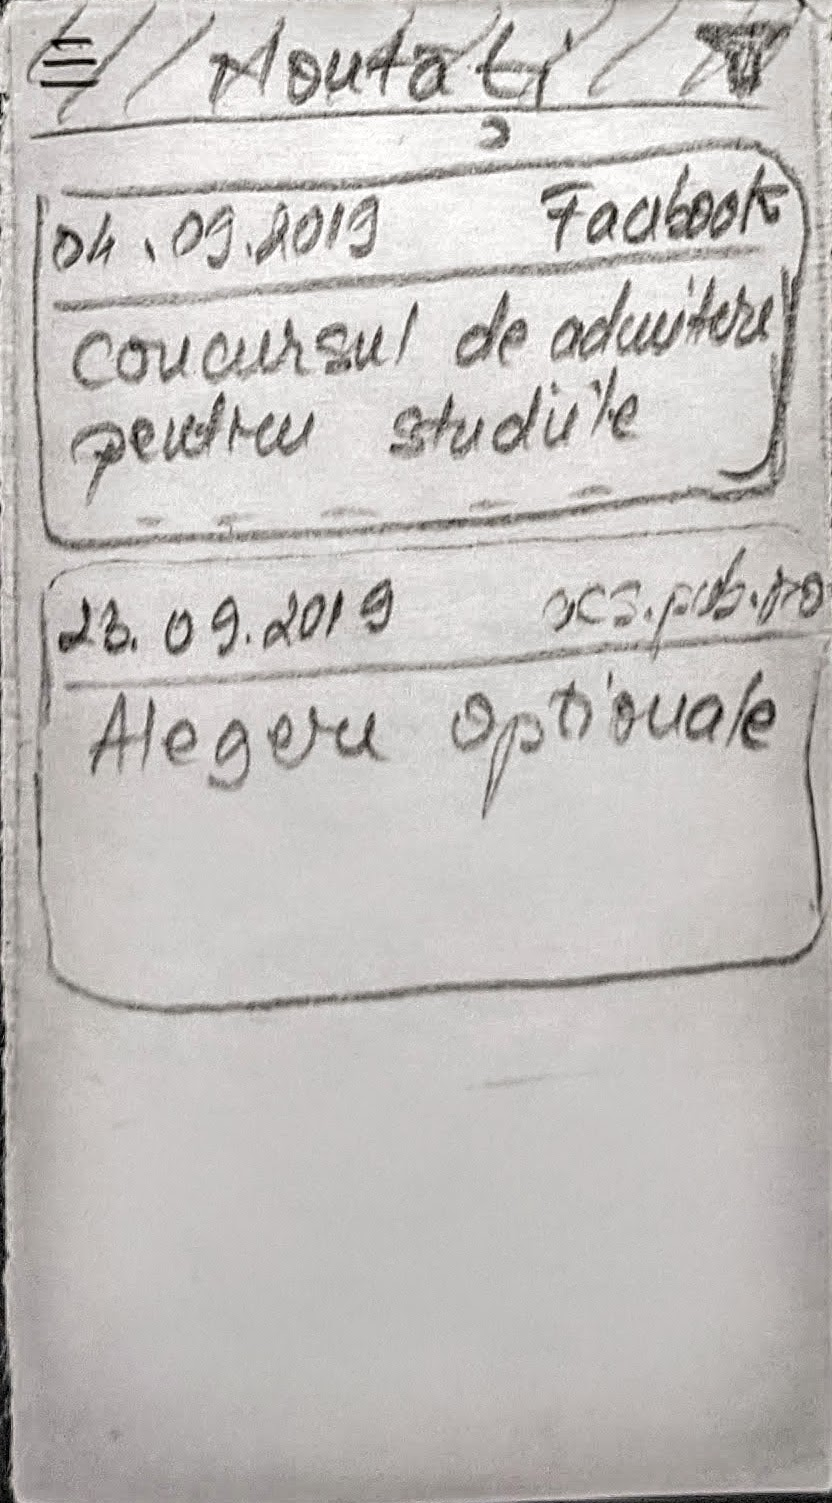
\includegraphics[height=0.279\textheight]{figures/app/paper/news.jpg}
         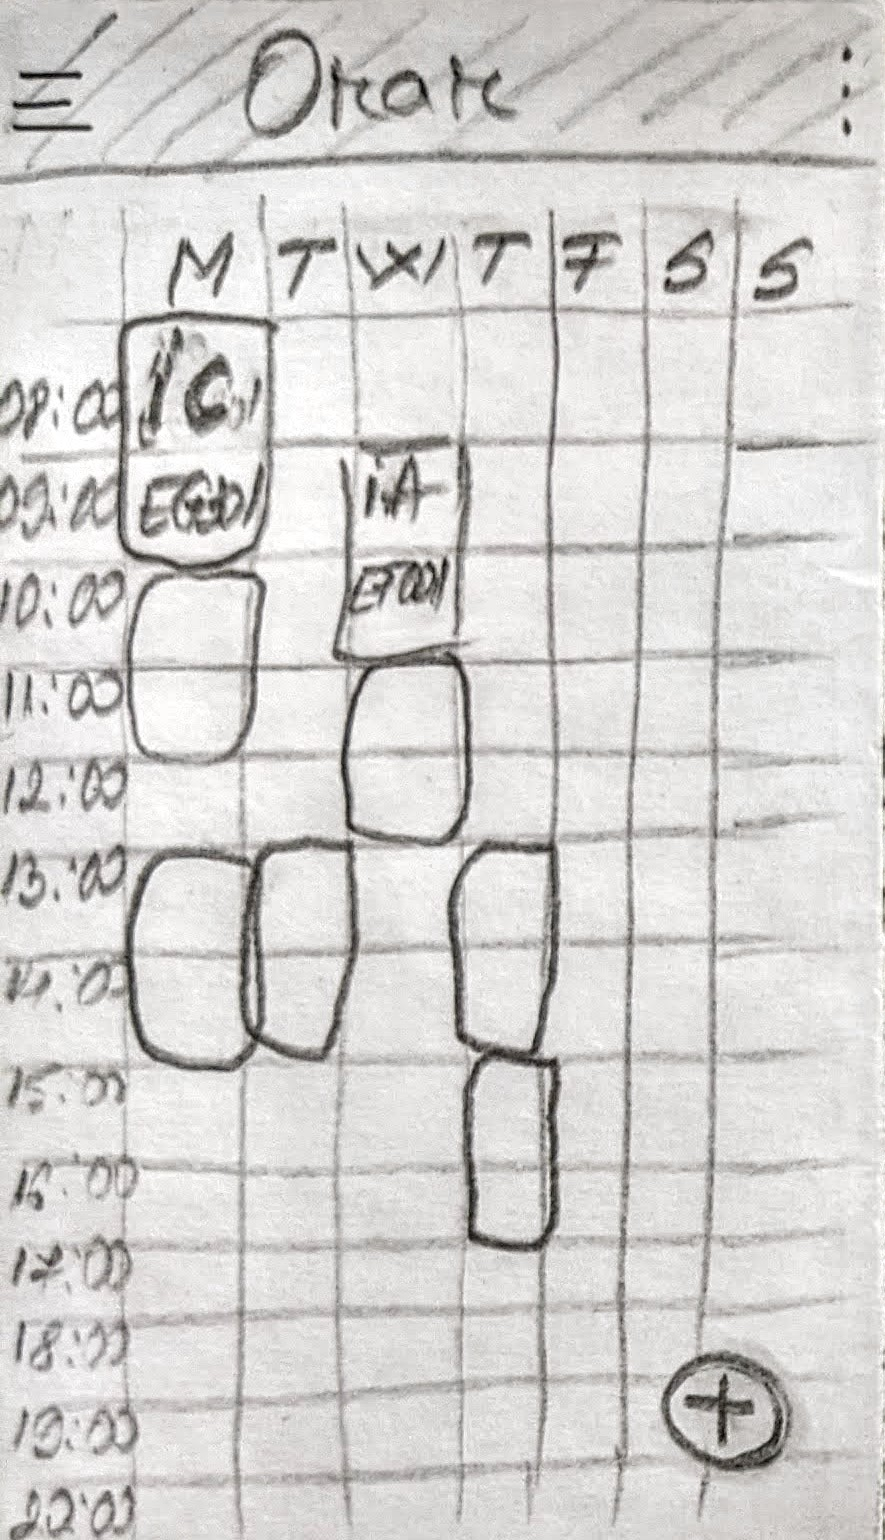
\includegraphics[height=0.279\textheight]{figures/app/paper/timetable.jpg}
         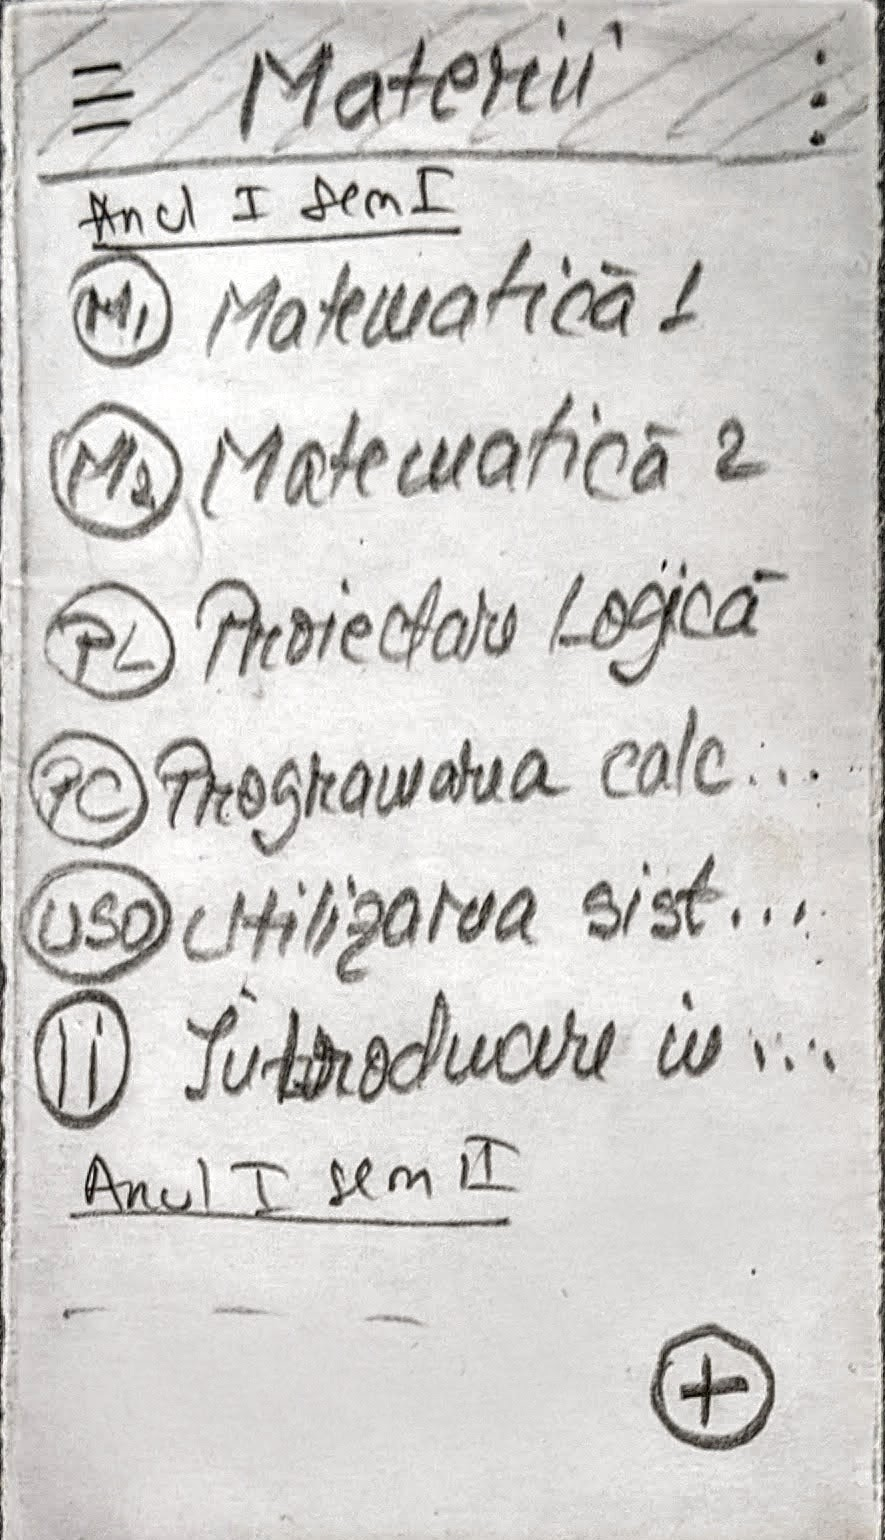
\includegraphics[height=0.279\textheight]{figures/app/paper/classes.jpg}
         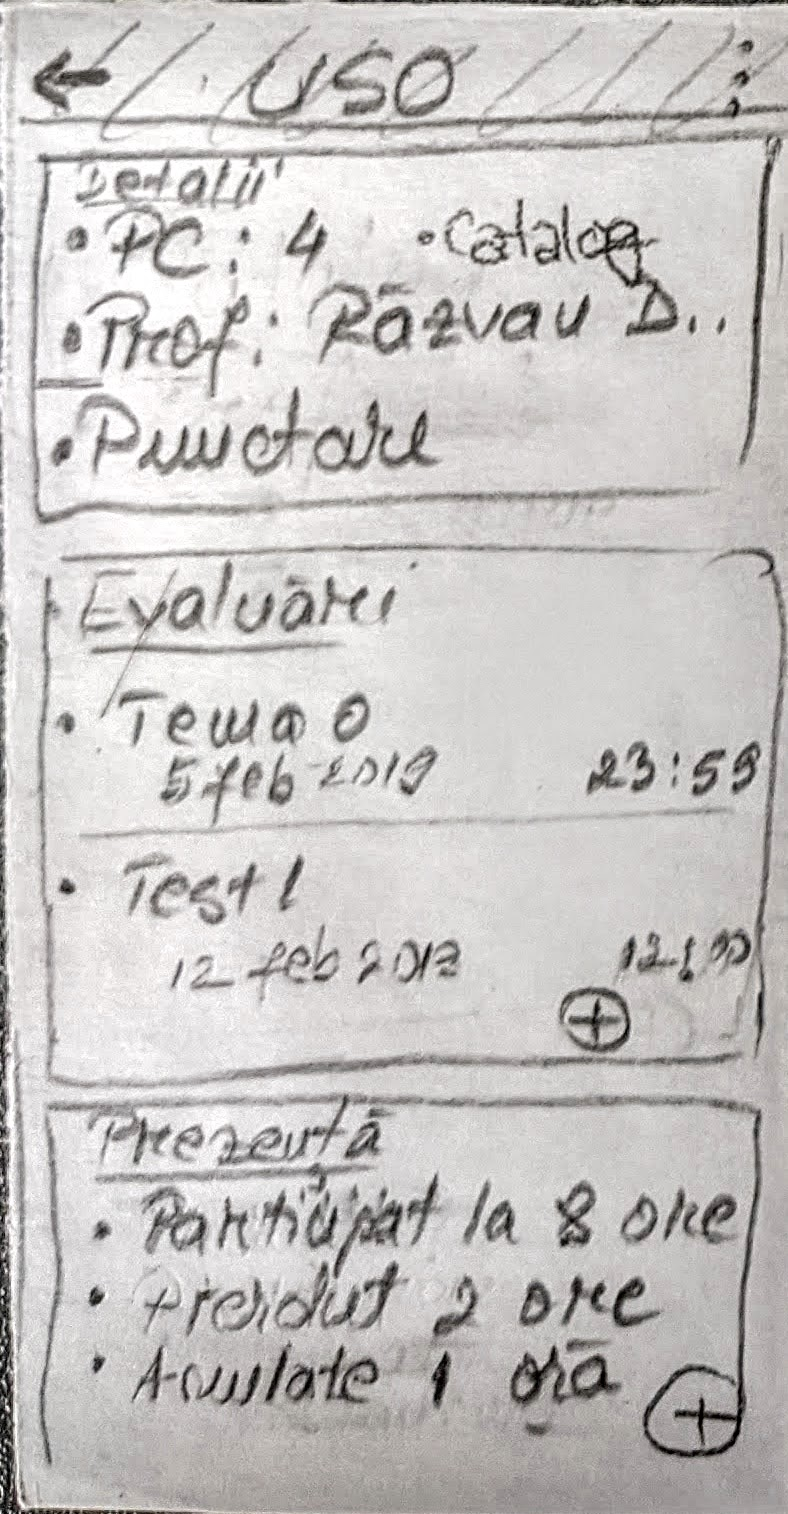
\includegraphics[height=0.279\textheight]{figures/app/paper/class_info.jpg}
         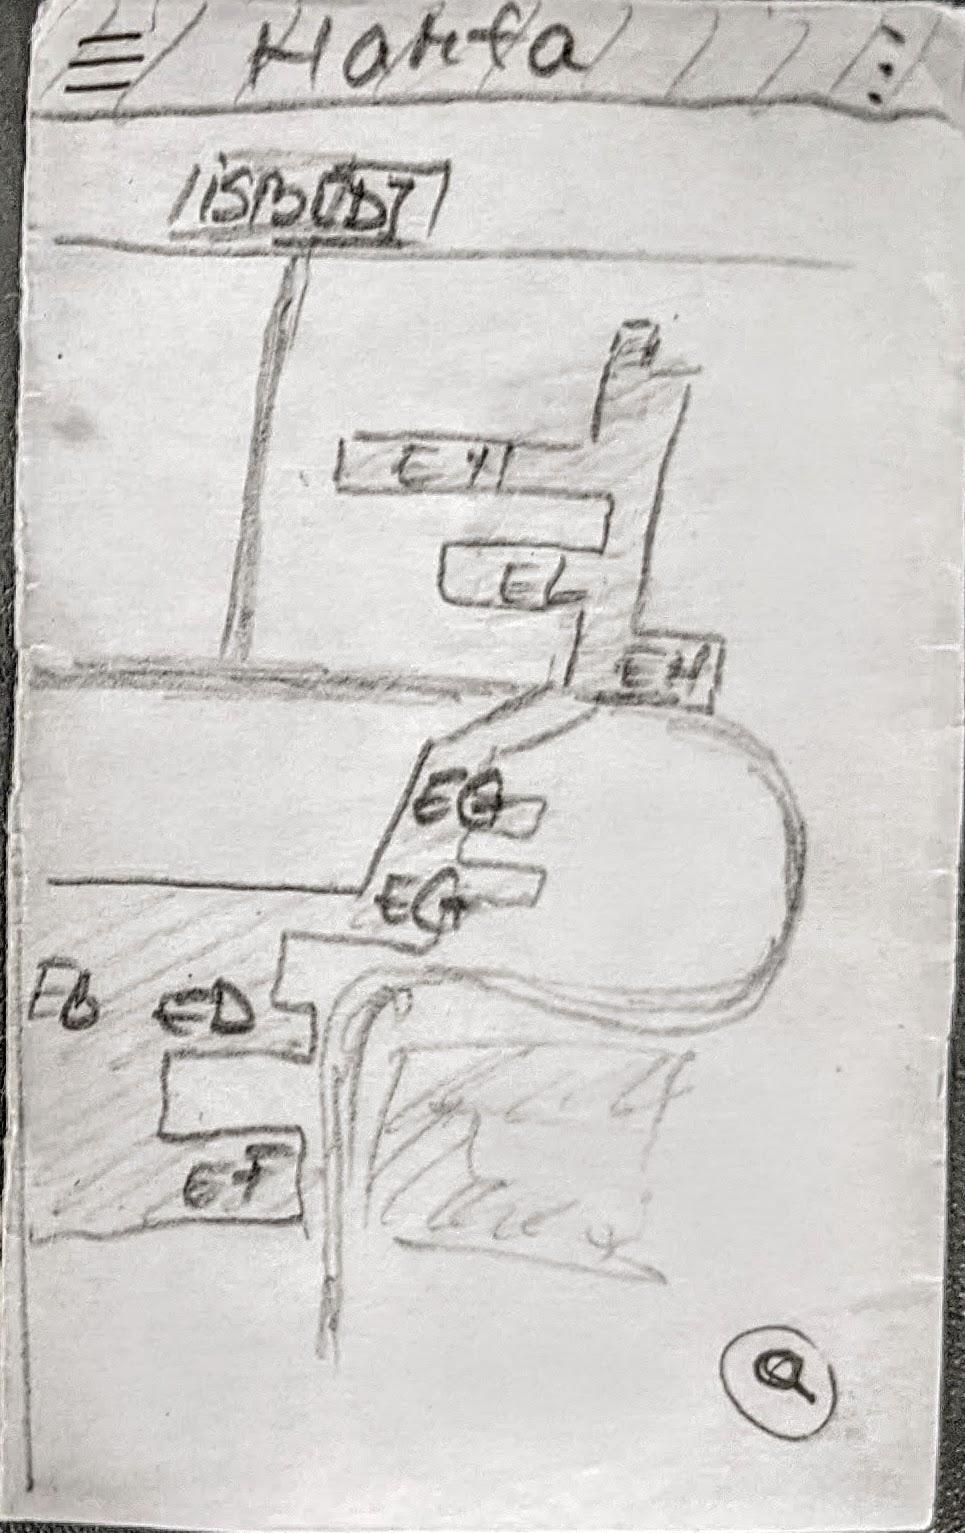
\includegraphics[height=0.279\textheight]{figures/app/paper/map.jpg}
    \caption{Paper prototype}
    \label{4:fig:paper_prototyping}
\end{figure}

\clearpage

Figure \ref{4:fig:paper_prototyping} shows the very first sketches of the application interface. The pages pictured, from left to right and top to bottom, are:
\begin{itemize}
    \setlength{\topsep}{0.5pt}
    \setlength{\itemsep}{0.5pt}
    \setlength{\parsep}{0.5pt}
    \item the login page the user would see when first opening the app
    \item the Material\cite{google2020material}-style side drawer with the different pages in the app, available once the user logs in
    \item a list of the university's platforms, which would serve as the default page the user would see without accessing the drawer
    \item the "News" page with information from various sources, such as relevant Facebook pages and the official website
    \item the timetable, with a button to add a new event
    \item the list of classes, organized by year/semester, with a button to add a new class
    \item information about a class that a user would see when clicking on an event or class
    \item the map of the campus, with a button to search for a specific location
\end{itemize}

\subsection{Feedback} \label{4:paper_feedback}

To find out what students would think about this initial concept, we organized a focus group with about 15 students and presented each of them the workflow of our application. Regarding \textbf{authentication}, we have received feedback regarding the need for a profile page for the user. The possibility for a user to use the app without having to authenticate was also mentioned. Multiple students pointed out that having the "Platforms" page as the default was counter-intuitive, and that a \textbf{designated "Home" page} would be a better solution. When asked what they think this homepage should contain, they suggested quick actions and upcoming events; in other words, an overview at a glance of the other pages within the app.

Some students pointed out that the homework-type events should have both \textbf{a soft and a hard deadline} associated with them, as is the norm in the faculty. Additionally, they wanted to see how the process of adding a new event would work.

\section{Permissions \& moderation system} \label{4:permissions}

\subsection{The need for moderation} \label{4:permissions_need}

As mentioned in section \ref{2:mix_and_match}, any collaborative system involving more than a few users requires some form of moderation\cite{roberts2019behind}. This system is meant to ensure that content stays accurate and up-to-date and avoid offensive/inappropriate content.

Based on the categories described by a \textit{Bridged.co} writer\cite{bridged2019moderation}, we will be using a mixture of \textbf{pre-moderation} and \textbf{reactive moderation}, meaning that content will be verified before appearing on the platform, and users can report or flag content that they believe to be inappropriate after it has been posted.

Since the platform should eventually be self-sustainable, without the need of constant involvement from the developer in content moderation (as is the case for the nonscalable solution of the application \textit{Politehnik}, described in section \ref{2:existing_apps_timetable}), we need a way to offer students the ability to moderate content on the platform themselves. This situation begs the question - how do we decide who should have the right to moderate content, and who should not?

\subsection{Permission levels} \label{4:permissions_levels}

To establish who should have certain rights, we need to define the rights that are to be granted. We have designed a permission-level system, where each user has a permission number, which indicates what they can do within the application. Each level includes the permissions of lower levels.

\begin{itemize}
    \setlength{\topsep}{0.5pt}
    \setlength{\itemsep}{0.5pt}
    \setlength{\parsep}{0.5pt}
    \item \textbf{0} - no special permissions; user can read public (already filtered) content and add private content or make suggestions
    \item \textbf{1} - helper level; user can view suggestions made by other people and vote up/down depending on whether they believe the suggestion to be appropriate or not
    \item \textbf{2} - basic moderator level; user can approve suggestions (an approved suggestion would be made public) and post content directly (without needing review); they can only delete content they posted or approved
    \item \textbf{3} - complete moderator level; user can dismiss suggestions (dismissed suggestions would be deleted from the suggestions page and no longer visible to anyone) and delete content added by anyone
    \item \textbf{4} - administrator level; user can change other users' permission level
\end{itemize}

\subsection{Assigning permissions} \label{4:permissions_assigning}

By default, any new user would have the first permission level (0). Initially, only the developers would have level 4, allowing them to assign special permissions to trusted students in their circle. Additionally, students who have a special status within the faculty (group/series representatives, certain members of student associations) can request to be granted level 2 to inform their fellow students easily.

In the future, a manually-defined permission system might prove not to be scalable. In this case, one potential solution would be for users' permissions to gradually increase as they contribute quality content to the platform (e.g., make/vote up suggestions that end up being approved, vote down suggestions that end up being dismissed). This system could be implemented into the application in a \textbf{gamified} manner (e.g., unlocking achievements and earning points by doing specific actions). Game-like platforms have a history of motivating students to participate actively. One such example within the faculty is \textit{World of USO}\footnote{https://wouso.cs.pub.ro/}, a competitive knowledge game played throughout the first semester by first-year students for the Introduction to Operating Systems (USO) class.

\section{Wireframe} \label{4:wireframe}

\subsection{Prototype} \label{4:wireframe_prototype}

Following the focus group, we noted the feedback and created a more detailed, interactive (clickable) wireframe using Balsamiq\footnote{https://balsamiq.com/}. We re-drew the login page (fig. \ref{4:fig:balsamiq_login}), drawer (fig. \ref{4:fig:balsamiq_menu}) and websites page (fig. \ref{4:fig:balsamiq_websites}), and introduced a home page (fig. \ref{4:fig:balsamiq_home}), as suggested by the feedback described in section \ref{4:paper_feedback}. The latter includes a list of frequently accessed websites, as well as upcoming events and tasks.

\begin{figure}[!ht]
    \centering
    \begin{minipage}[b]{0.25\textwidth}
        \captionsetup{justification=centering}
        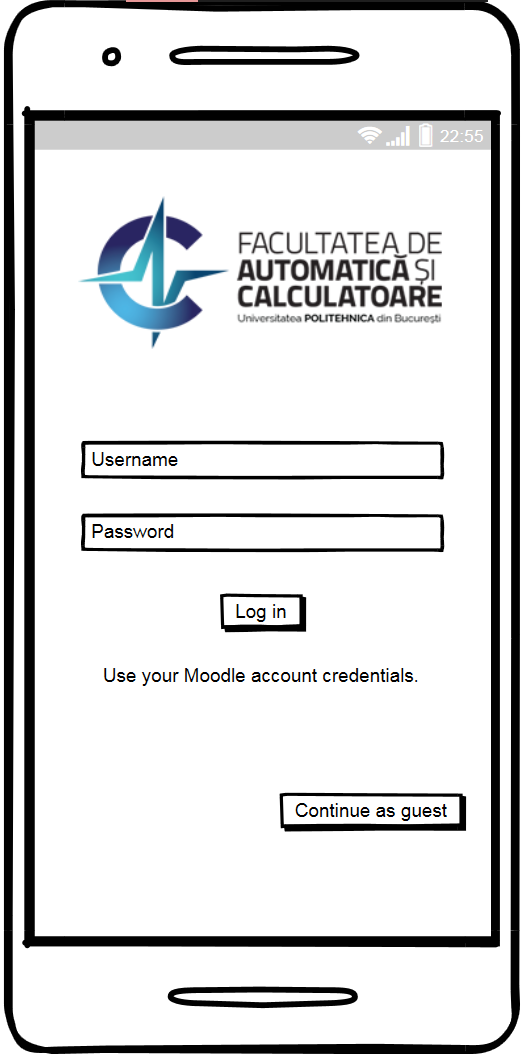
\includegraphics[width=\textwidth]{figures/app/balsamiq/login.png}
        \caption{Login page wireframe}
        \label{4:fig:balsamiq_login}
    \end{minipage}
    \hfill
    \begin{minipage}[b]{0.26\textwidth}
        \captionsetup{justification=centering}
        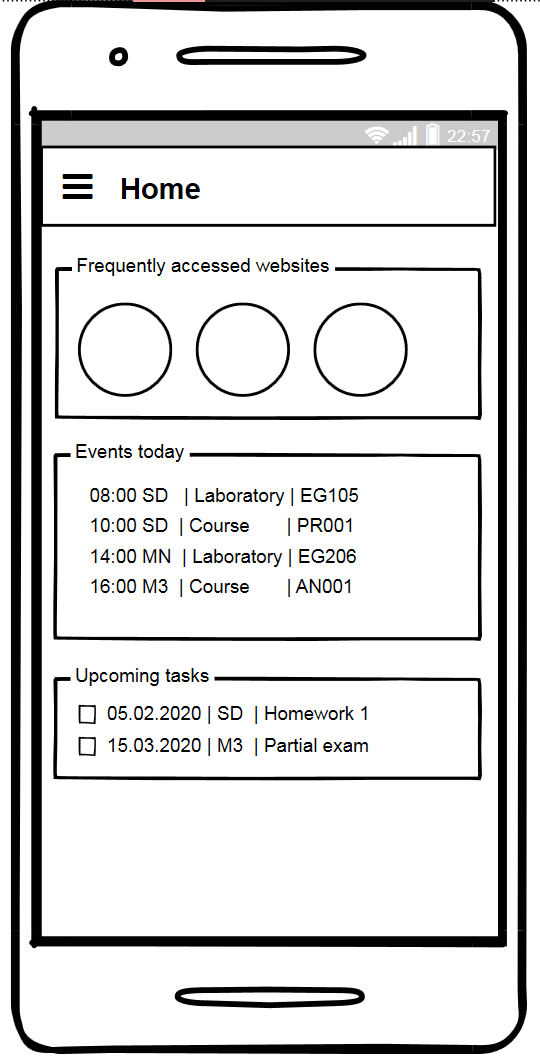
\includegraphics[width=\textwidth]{figures/app/balsamiq/home.png}
        \caption{Home page wireframe}
        \label{4:fig:balsamiq_home}
    \end{minipage}
    \hfill
    \begin{minipage}[b]{0.26\textwidth}
        \captionsetup{justification=centering}
        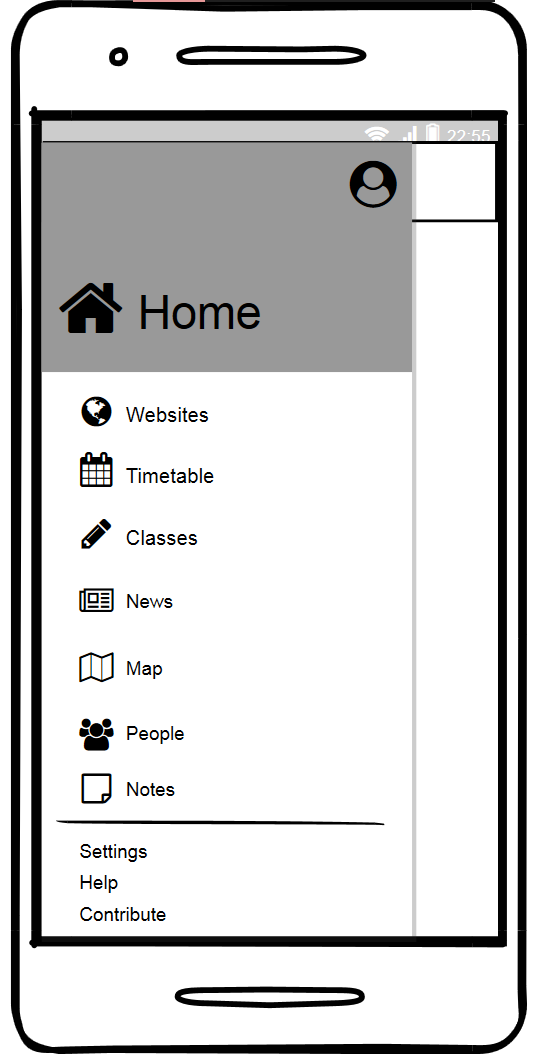
\includegraphics[width=\textwidth]{figures/app/balsamiq/drawer.png}
        \caption{Menu wireframe}
        \label{4:fig:balsamiq_menu}
    \end{minipage}
\end{figure}

We also re-drew the news page (fig. \ref{4:fig:balsamiq_news}) and added a visualization of the filtering option for this page.

\begin{figure}[!ht]
    \centering
    \begin{minipage}[t]{0.26\textwidth}
        \captionsetup{justification=centering}
        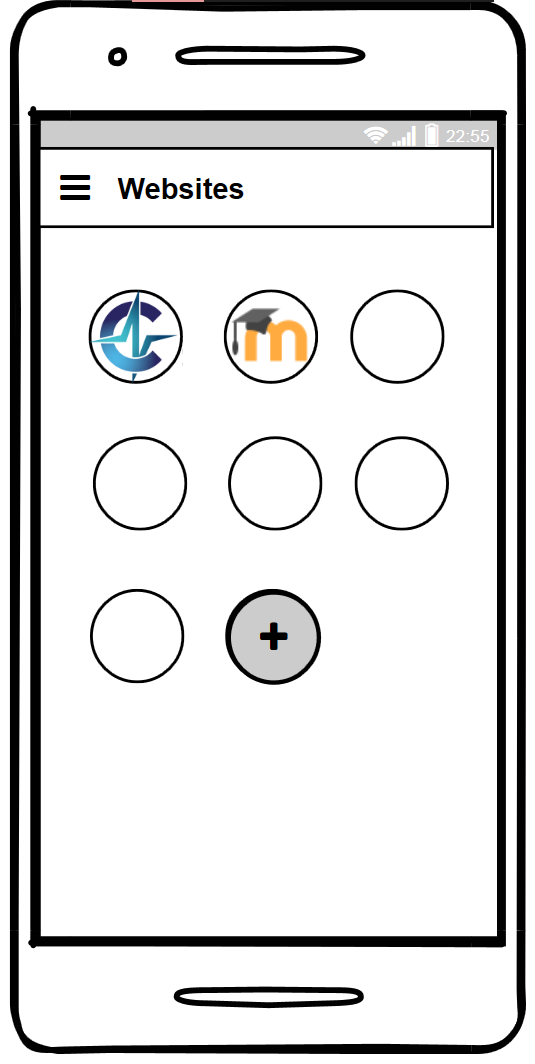
\includegraphics[width=\textwidth]{figures/app/balsamiq/websites.png}
        \caption{Websites page wireframe}
        \label{4:fig:balsamiq_websites}
    \end{minipage}
    \hfill
    \begin{minipage}[t]{0.54\textwidth}
        \captionsetup{justification=centering}
        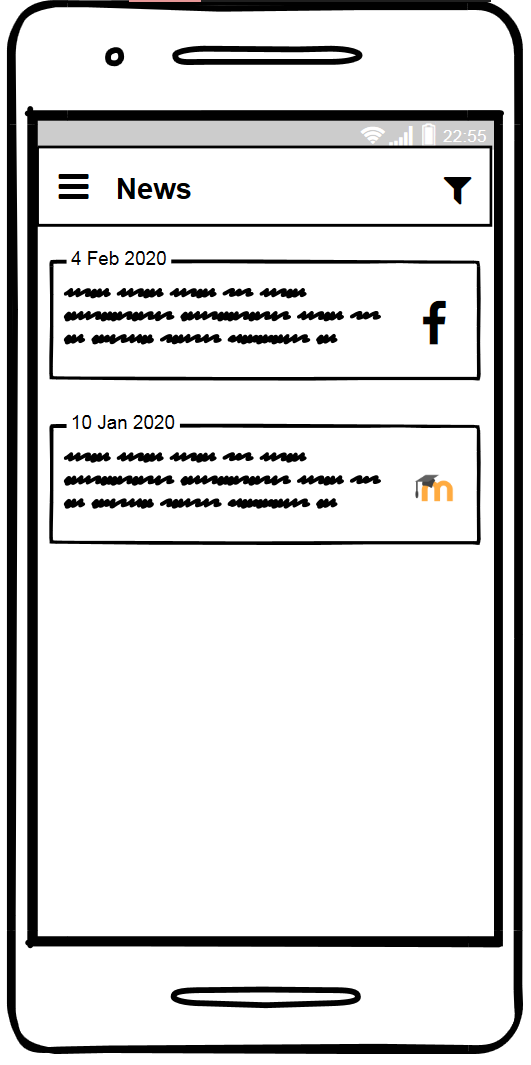
\includegraphics[width=0.485\textwidth]{figures/app/balsamiq/news.png}
        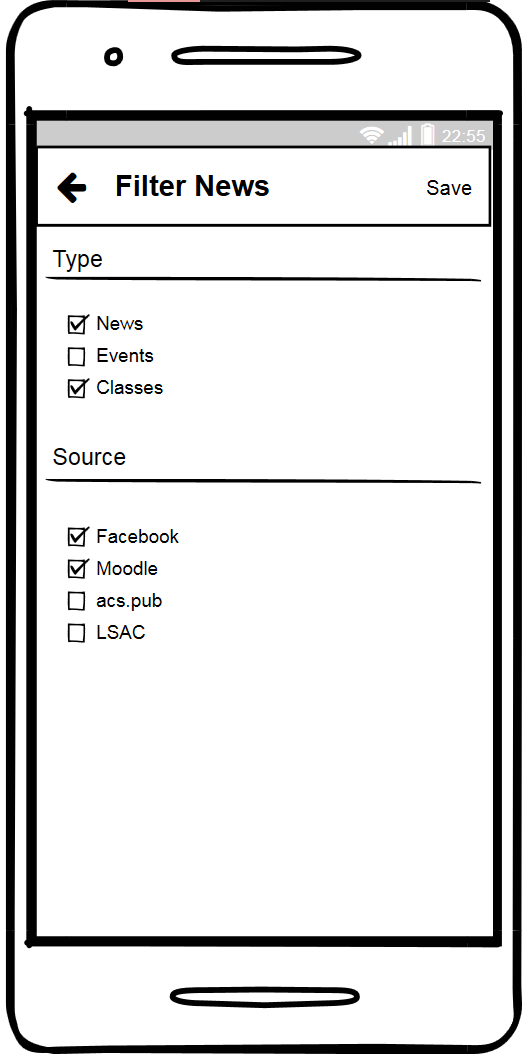
\includegraphics[width=0.49\textwidth]{figures/app/balsamiq/filter_news.png}
        \caption{News page wireframe}
        \label{4:fig:balsamiq_news}
    \end{minipage}
\end{figure}

Additionally, we added the profile page (fig. \ref{4:fig:balsamiq_profile}) requested by the feedback. It includes a potential presentation of the gamification feature suggested in section \ref{4:permissions_assigning}. This concept displays the current level of the user as well as the requirements for progressing to the next one.

We also drew the "People" page containing professor and student information (fig. \ref{4:fig:balsamiq_people}). It is pictured as a list of names and allows the user to click/tap a name to view more information about the person. It also allows filtering the list by type (student/professor).

\begin{figure}[!ht]
    \centering
    \begin{minipage}[t]{0.3\textwidth}
        \captionsetup{justification=centering}
        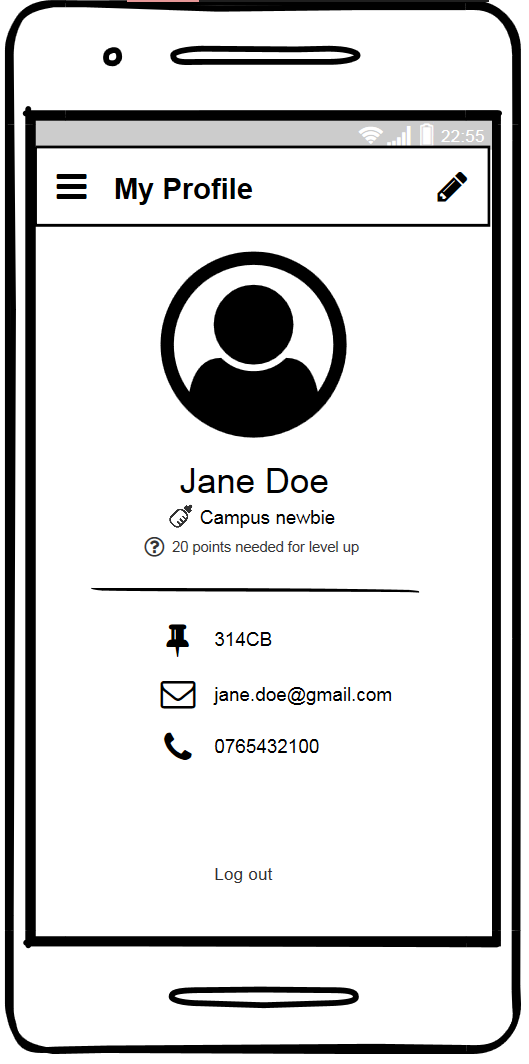
\includegraphics[width=\textwidth]{figures/app/balsamiq/profile.png}
        \caption{Profile page wireframe}
        \label{4:fig:balsamiq_profile}
    \end{minipage}
    \hfill
    \begin{minipage}[t]{0.63\textwidth}
        \captionsetup{justification=centering}
        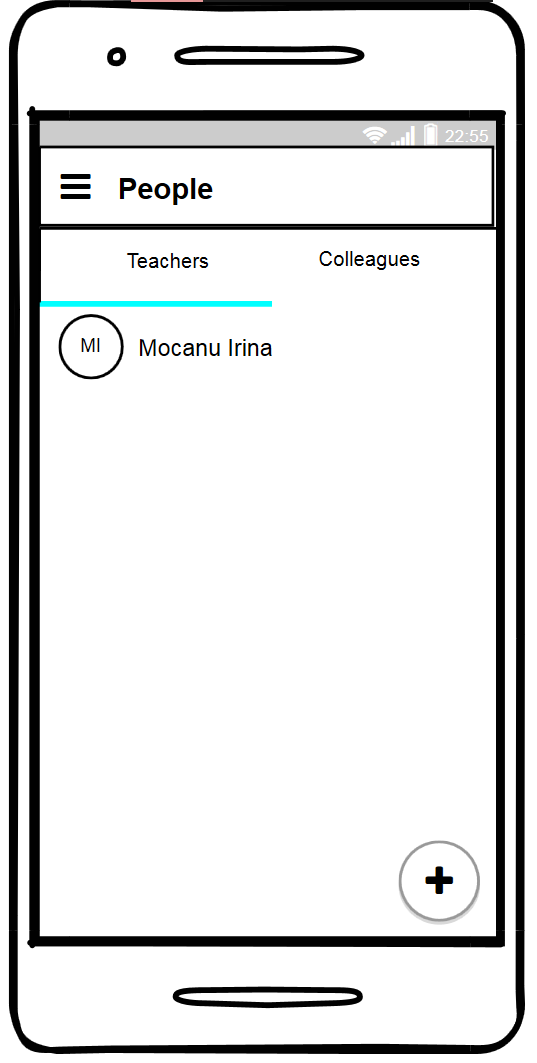
\includegraphics[width=0.485\textwidth]{figures/app/balsamiq/people.png}
        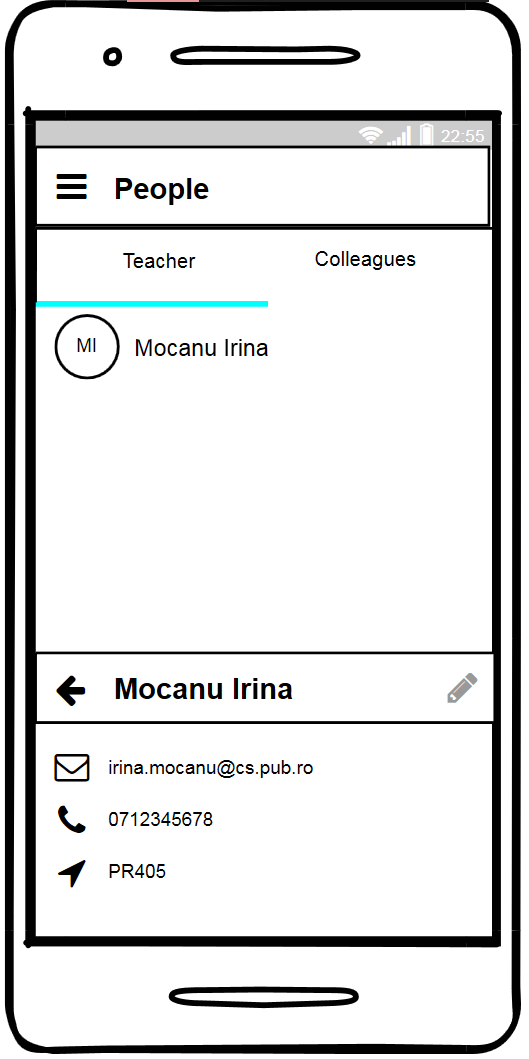
\includegraphics[width=0.48\textwidth]{figures/app/balsamiq/teacher.png}
        \caption{People page wireframe}
        \label{4:fig:balsamiq_people}
    \end{minipage}
\end{figure}

Finally, we re-designed the classes and class information pages (fig. \ref{4:fig:balsamiq_classes}) and added visualizations for the filtering mechanism as well as the entire process of adding a new event to a class (fig. \ref{4:fig:balsamiq_events}), as requested by the feedback.

Adding an event can be done by either manually inputting all data for the event (such as the name, class, and deadlines for homework) or using an event that somebody else has already created. Existing events can be voted up or down. They would be automatically voted up if a user chooses to add it to their calendar in the application.

\clearpage

\begin{figure}[!ht]
    \centering
     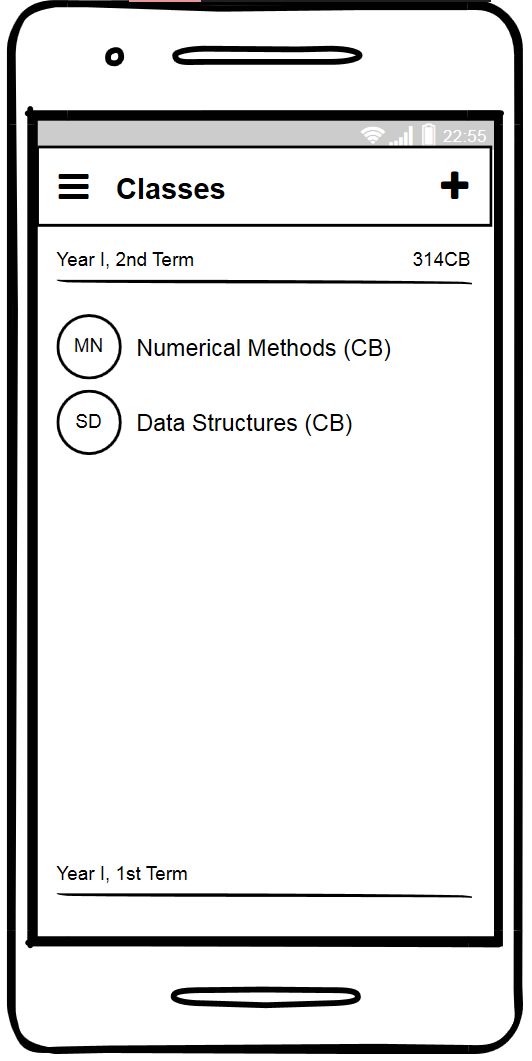
\includegraphics[width=0.32\textwidth]{figures/app/balsamiq/classes.png}
     \hfill
     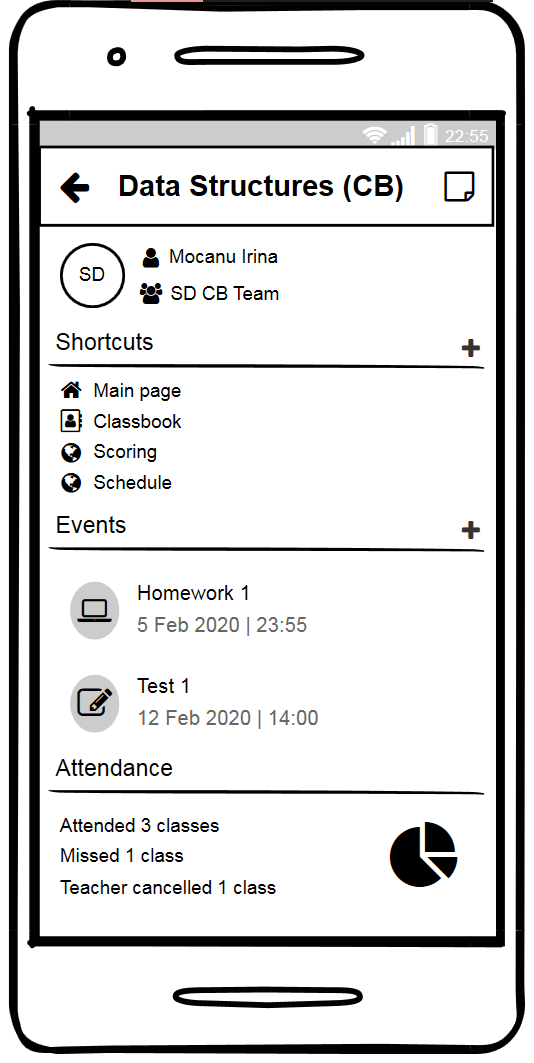
\includegraphics[width=0.32\textwidth]{figures/app/balsamiq/class_info.png}
     \hfill
     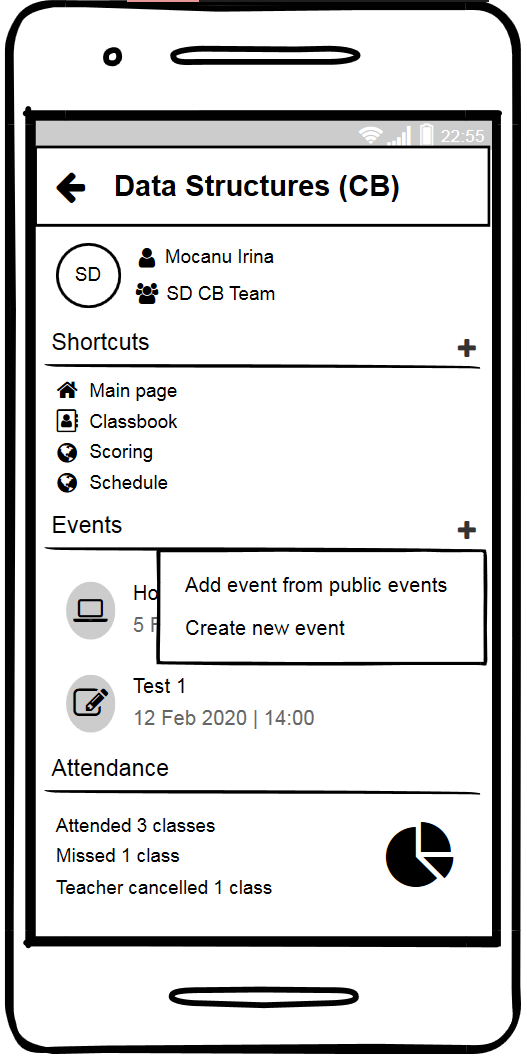
\includegraphics[width=0.32\textwidth]{figures/app/balsamiq/add_event.png}
    \caption{Classes page wireframe}
    \label{4:fig:balsamiq_classes}
\end{figure}

\begin{figure}[!ht]
    \centering
     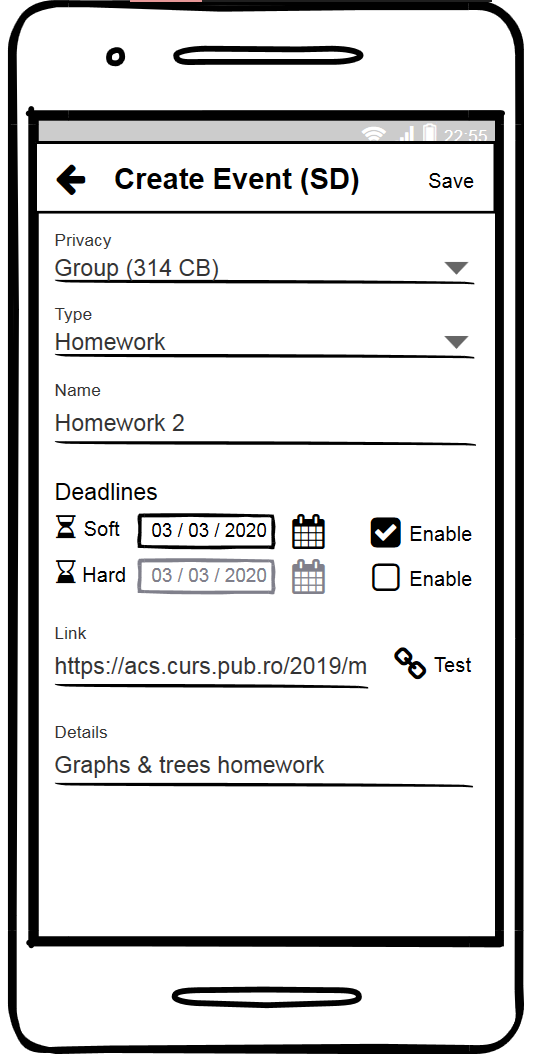
\includegraphics[width=0.32\textwidth]{figures/app/balsamiq/create_event.png}
     \hfill
     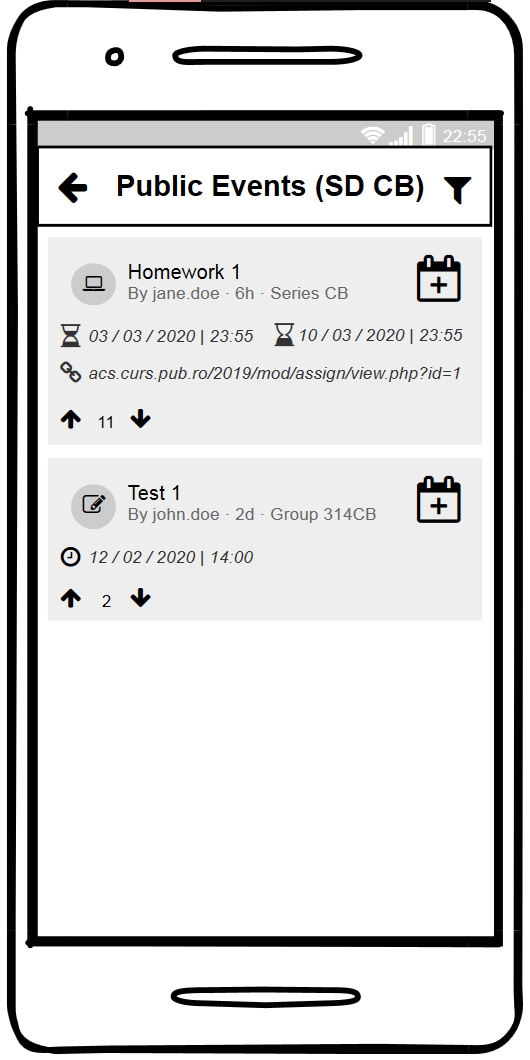
\includegraphics[width=0.32\textwidth]{figures/app/balsamiq/public_events.png}
     \hfill
     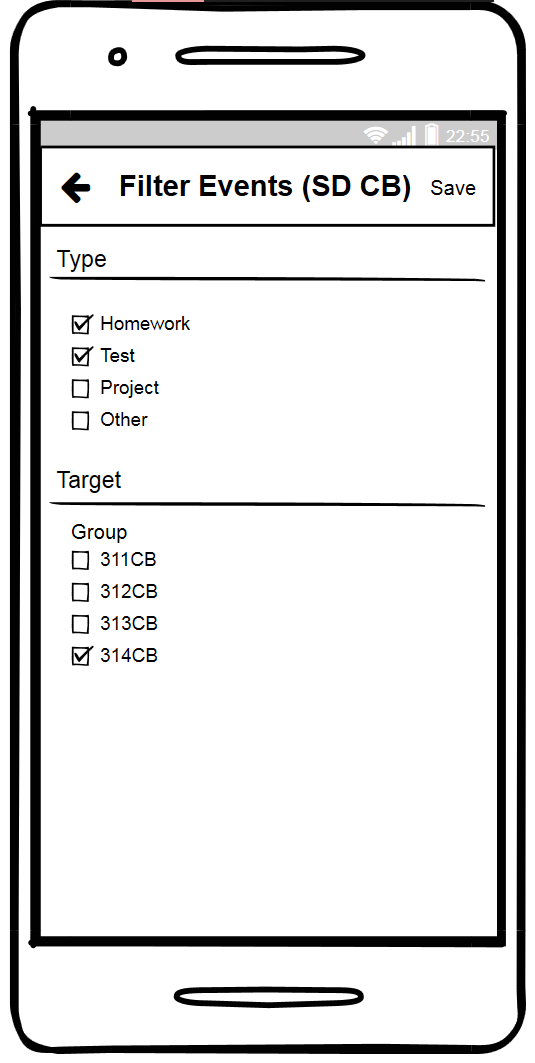
\includegraphics[width=0.32\textwidth]{figures/app/balsamiq/filter_events.png}
    \caption{Events page wireframe}
    \label{4:fig:balsamiq_events}
\end{figure}

\subsection{Feedback} \label{4:wireframe_feedback}

We asked ten students from different years to test this prototype and share their experiences. The feedback we received was very positive, with all students showing excitement about the application's features.

The students who have iOS devices pointed out that the design style is more appropriate for Android than iOS devices, which was to be expected since the main inspiration for the prototype was an Android application which uses Material Design\cite{google2020material} (\textit{School Assistant}).

Some students noted that a voting system on events could be abused since the user can ask their colleagues for votes.

\section{Final design} \label{4:final}

\subsection{Theme} \label{4:final_theme}

\begin{wrapfigure}{l}{0.14\columnwidth}
    \centering
    \captionsetup{justification=centering}
    
\includegraphics[width=0.14\columnwidth]{figures/logos/acs.png}
    \caption{\acrshort{acs} logo}
    \label{4:fig:acs_logo}
\end{wrapfigure}

For the final design, we created a dual theme (including dark \& light mode) that is inspired by the faculty logo (fig. \ref{4:fig:acs_logo}). The primary and secondary colors of the application are extracted from the logo and used for text, buttons as well as illustrations.

The font used in the application is Montserrat\footnote{https://fonts.google.com/specimen/Montserrat}. All icons are either Material Design icons\footnote{https://material.io/resources/icons/} or FontAwesome icons\footnote{https://fontawesome.com/icons/}. Illustrations are from the open-source unDraw\footnote{https://undraw.co/illustrations} gallery. All of the above are under open licenses and allow usage, modification, and redistribution.

\subsection{Pages} \label{4:pages}

For the sake of this paper, we will include only light theme / English screenshots of the most important pages in the application (figures \ref{4:fig:login} - \ref{4:fig:edit_event}).

We decided to drop the navigation drawer - hamburger menu (\faBars) combo (fig. \ref{4:fig:balsamiq_menu}) in favour of a bottom navigation bar (fig. \ref{4:fig:home}). This decision is mostly due to the drawer not being an accepted pattern on iOS. Additionally, in recent years, navigation drawers have sparked controversy\cite{verge2019controversy} in the context of mobile gestures and many applications - including Google applications like Google Maps\footnote{https://www.google.com/maps} - are removing the drawers entirely, opting for a bottom navigation bar instead.

The final design is otherwise fairly similar, \acrshort{ux}-wise, to the wireframe concept, but adds many \acrshort{ui} design elements such as a colour palette and illustrations on pages without a lot of content (such as the login/signup page - fig. \ref{4:fig:login} - and the settings page - \ref{4:fig:settings}).

\begin{figure}[!ht]
    \centering
    \begin{minipage}[b]{0.32\textwidth}
        \captionsetup{justification=centering}
        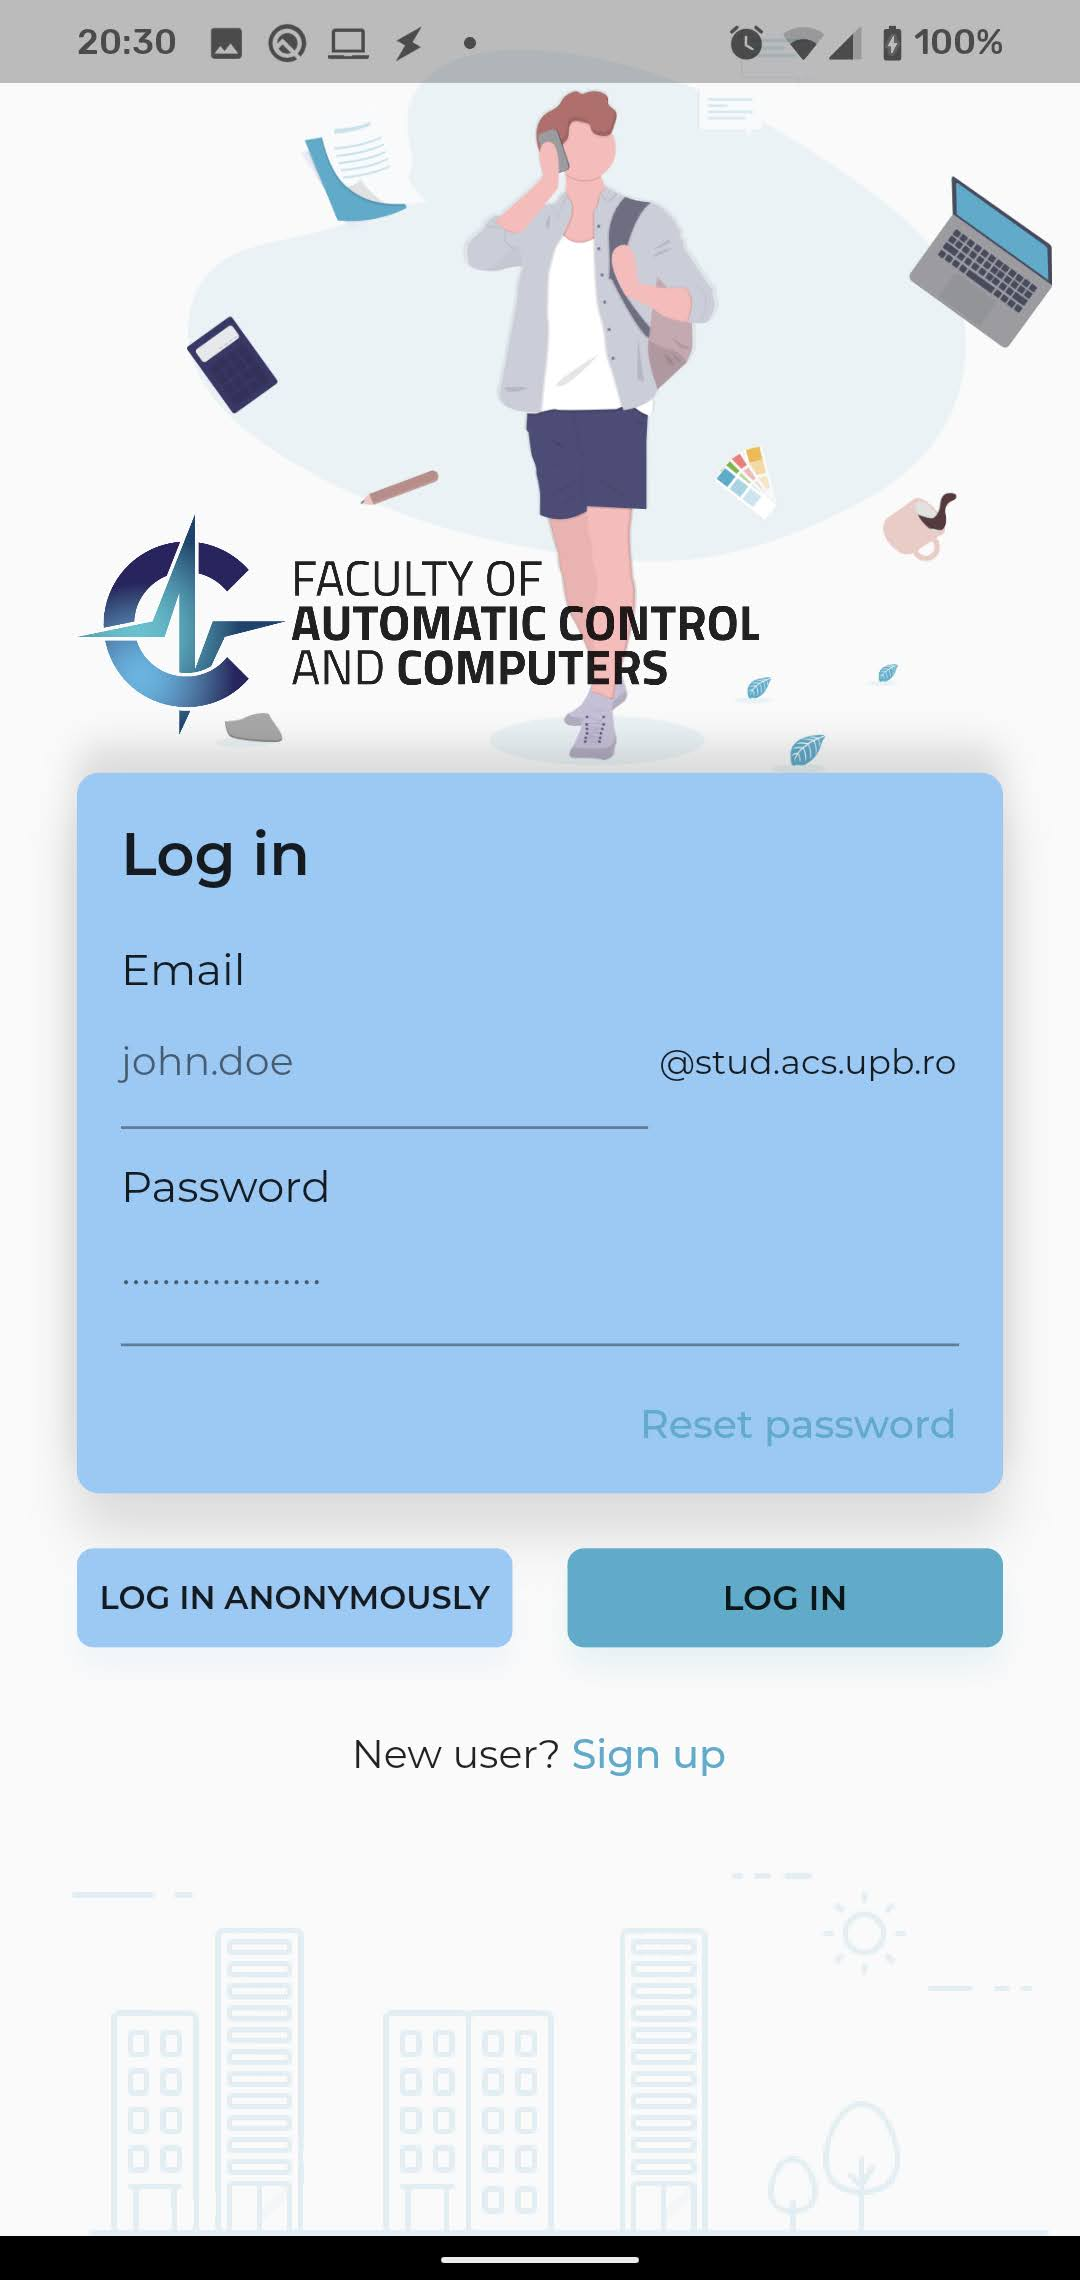
\includegraphics[width=\textwidth]{figures/app/flutter/login.jpg}
        \caption{Login page}
        \label{4:fig:login}
    \end{minipage}
    \hfill
    \begin{minipage}[b]{0.32\textwidth}
        \captionsetup{justification=centering}
        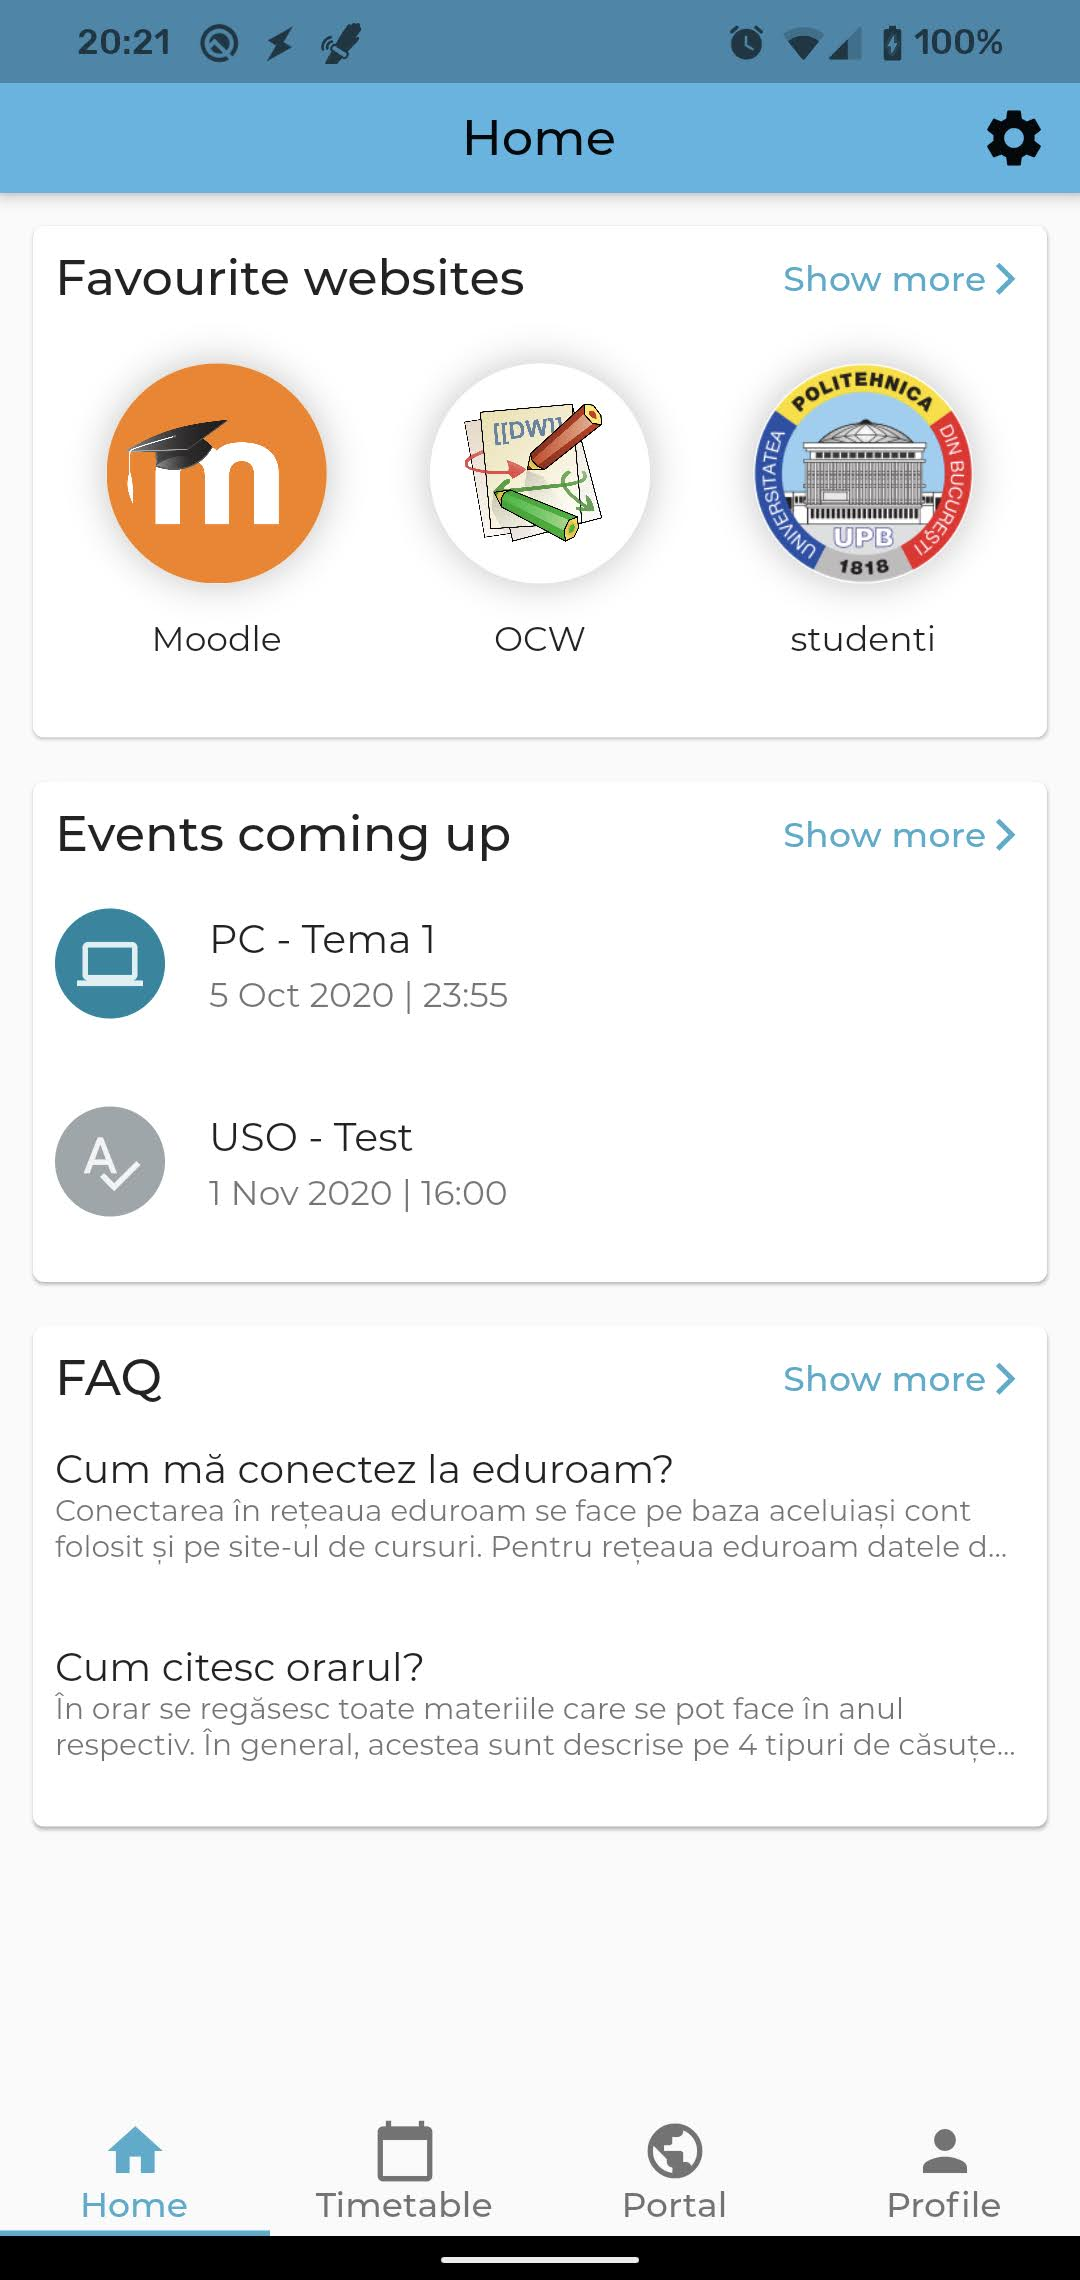
\includegraphics[width=\textwidth]{figures/app/flutter/home.jpg}
        \caption{Home page}
        \label{4:fig:home}
    \end{minipage}
    \hfill
    \begin{minipage}[b]{0.32\textwidth}
        \captionsetup{justification=centering}
        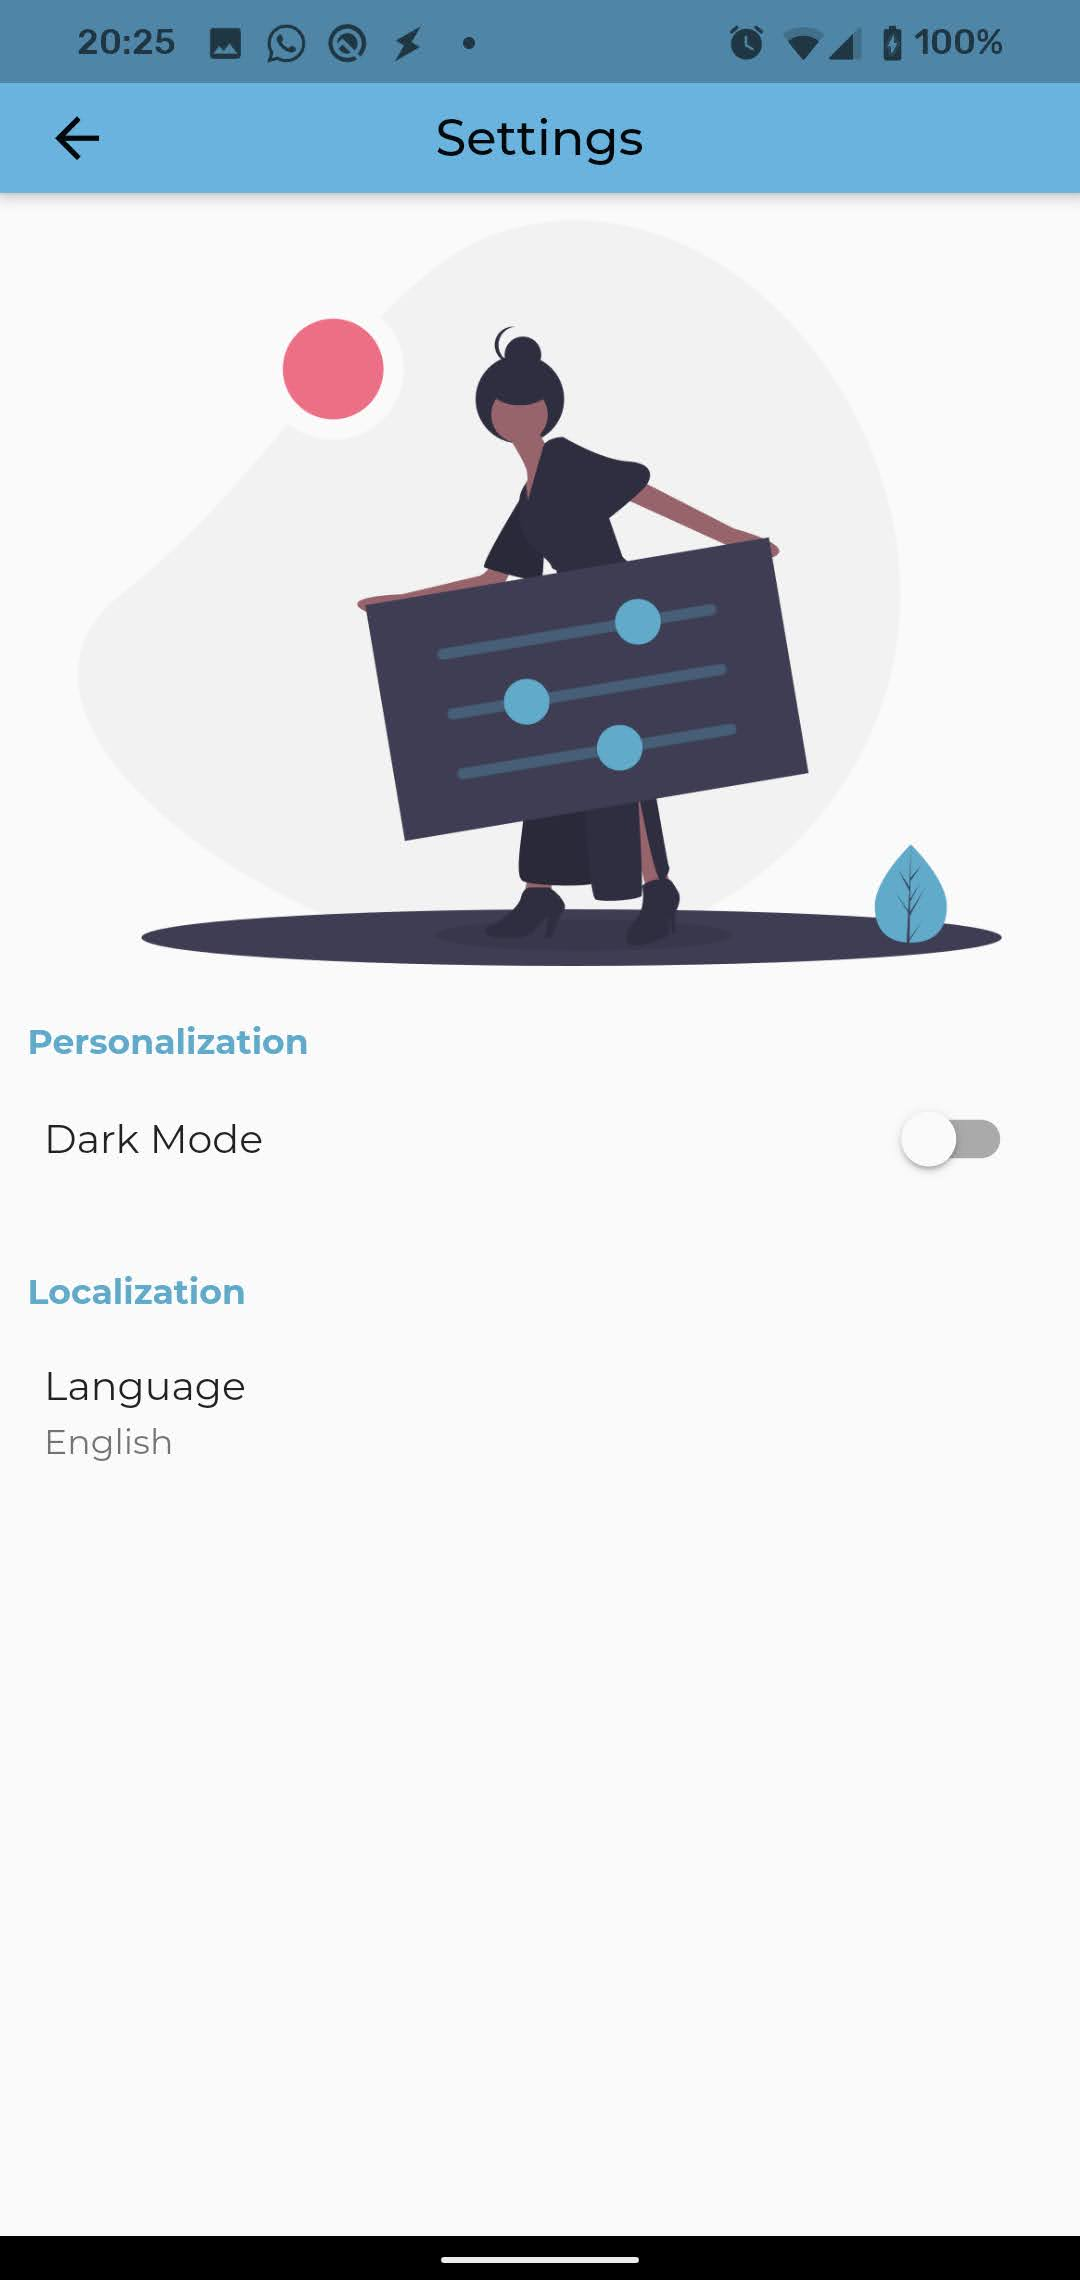
\includegraphics[width=\textwidth]{figures/app/flutter/settings.jpg}
        \caption{Settings page}
        \label{4:fig:settings}
    \end{minipage}
\end{figure}

The portal page (fig. \ref{4:fig:portal}) allows the user to tap a website to open a browser window following that link. Users can also add and edit websites (depending on their permissions, see section \ref{4:permissions_levels}), as shown in figure \ref{4:fig:website}, and filter them (fig. \ref{4:fig:filter}). The filter is a tree structure based on the student body structure described previously in section \ref{1:student_body_structure}), where students can select any number of nodes they would be interested in.

\clearpage

\begin{figure}[!ht]
    \centering
    \begin{minipage}[b]{0.26\textwidth}
        \captionsetup{justification=centering}
        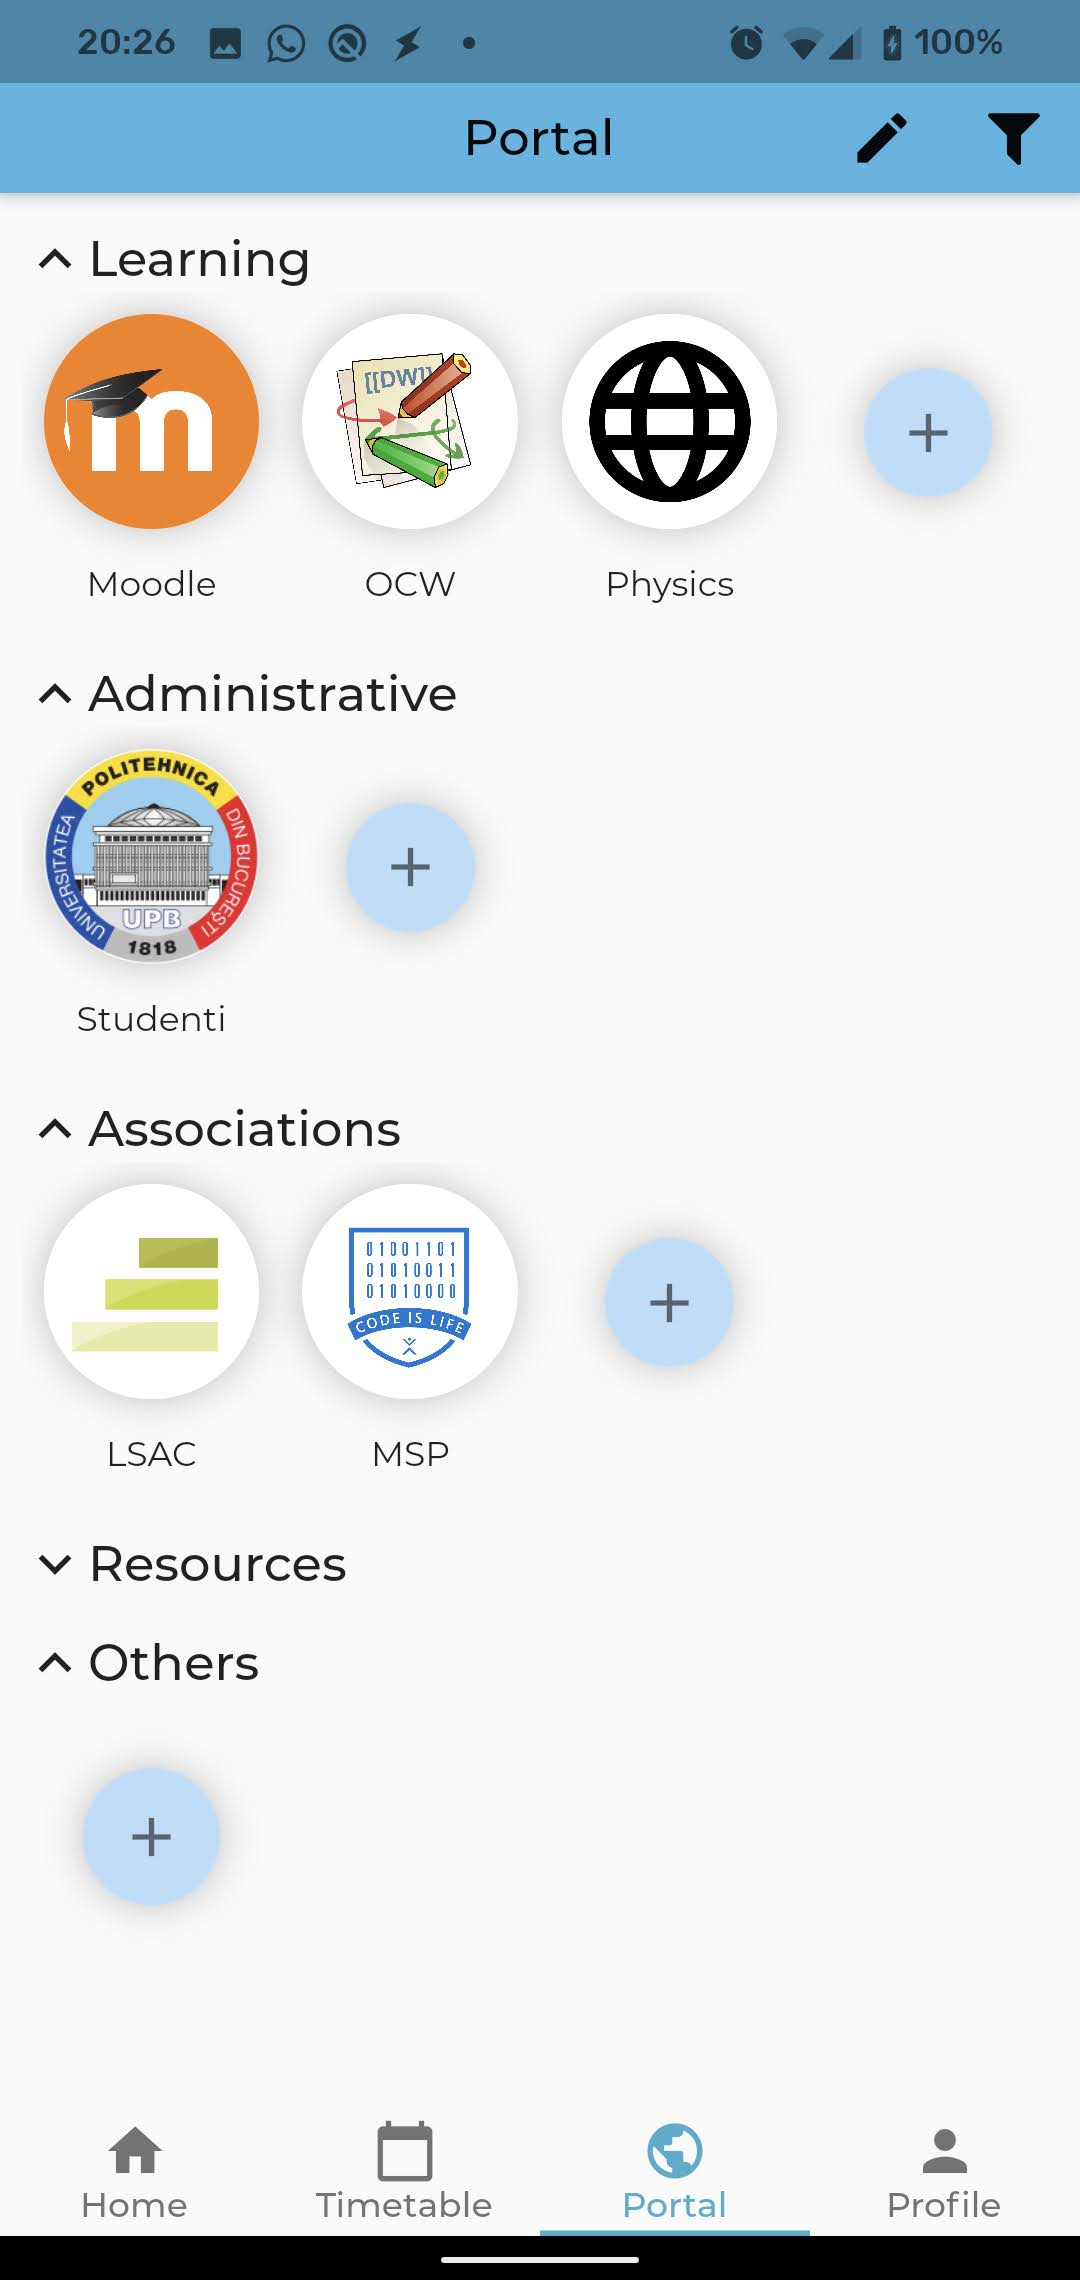
\includegraphics[width=\textwidth]{figures/app/flutter/portal.jpg}
        \caption{Portal page}
        \label{4:fig:portal}
    \end{minipage}
    \hfill
    \begin{minipage}[b]{0.26\textwidth}
        \captionsetup{justification=centering}
        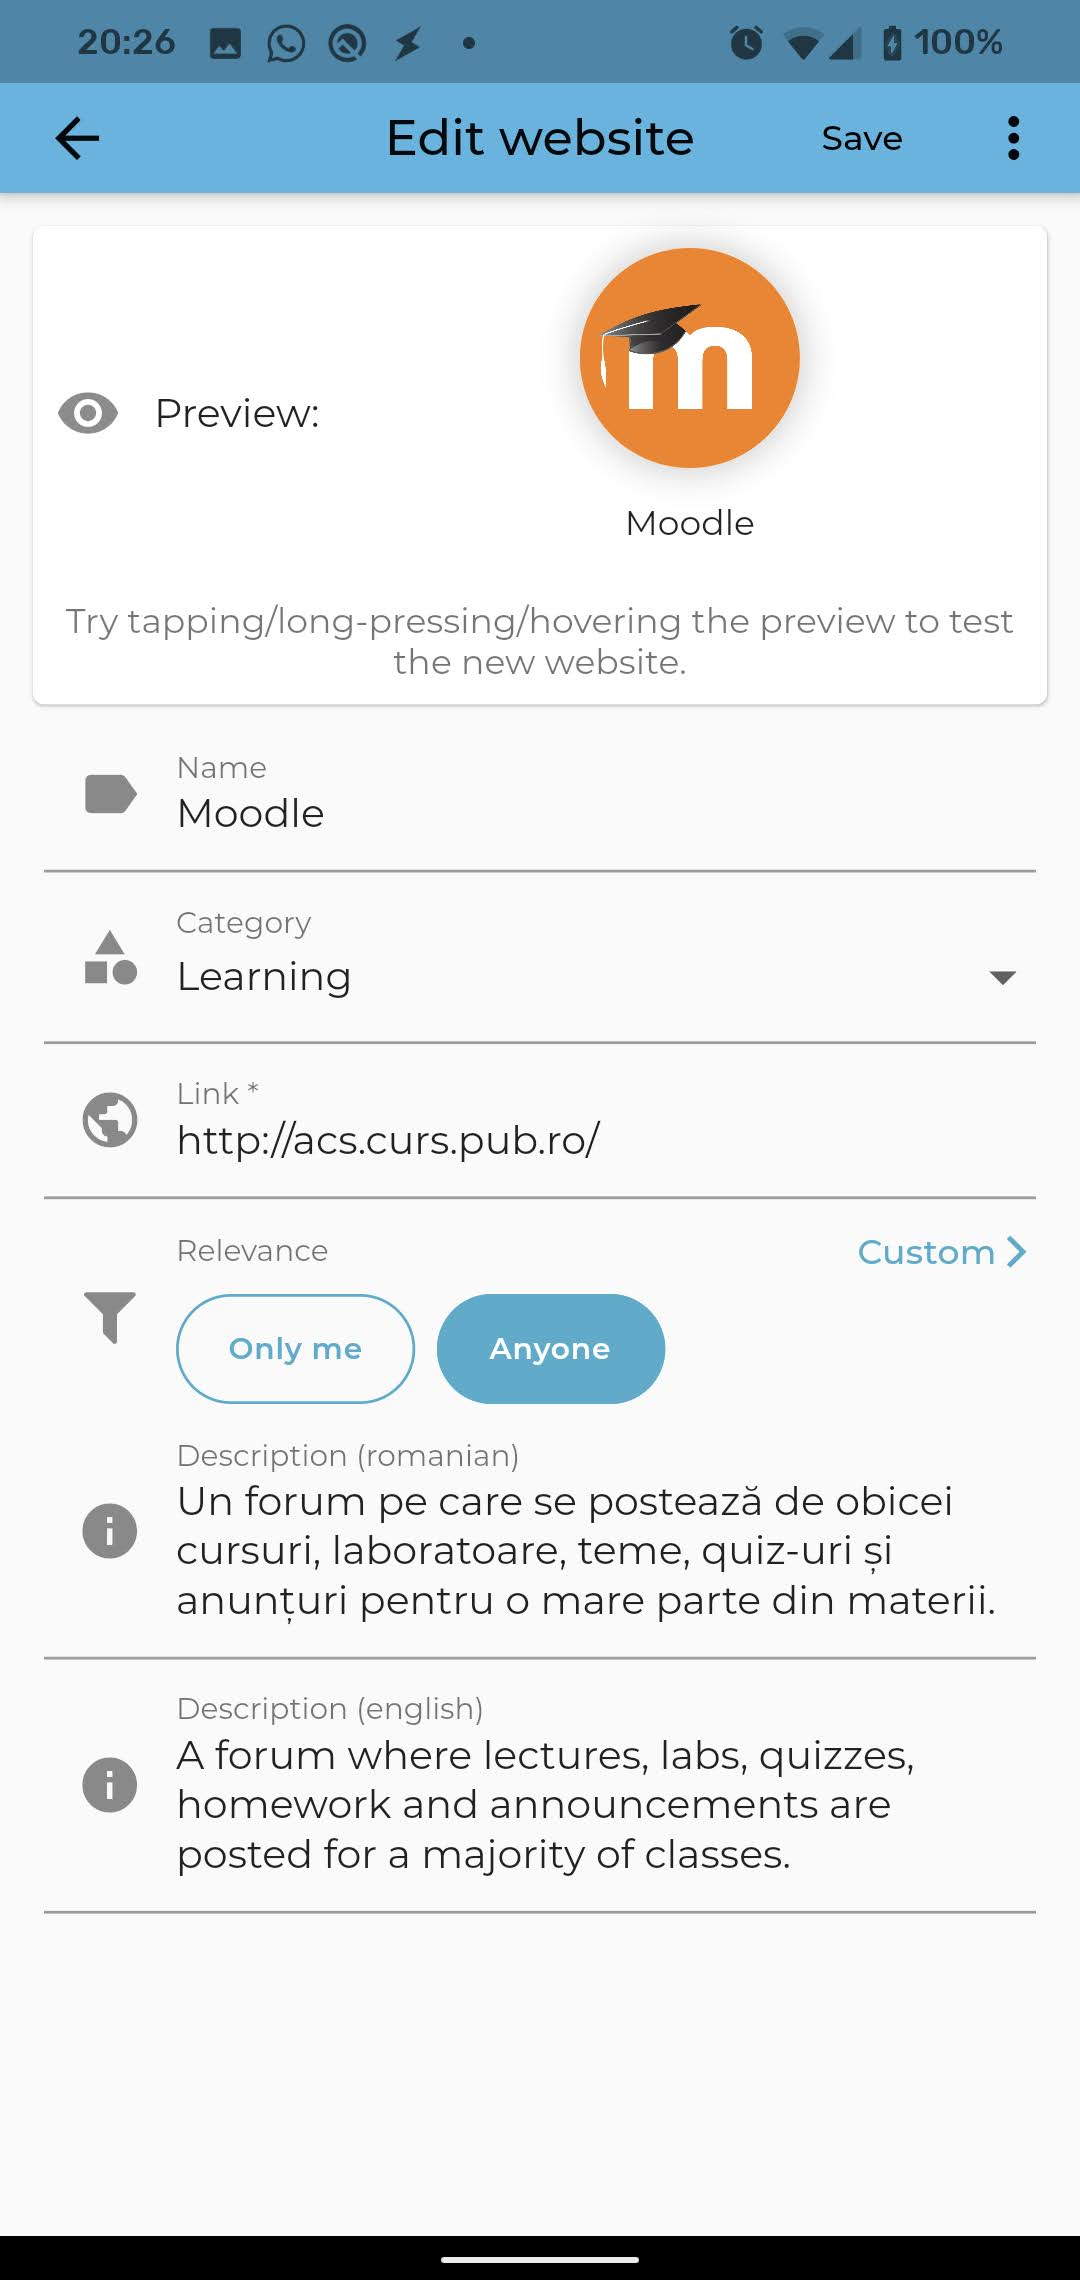
\includegraphics[width=\textwidth]{figures/app/flutter/website.jpg}
        \caption{Edit website page}
        \label{4:fig:website}
    \end{minipage}
    \hfill
    \begin{minipage}[b]{0.26\textwidth}
        \captionsetup{justification=centering}
        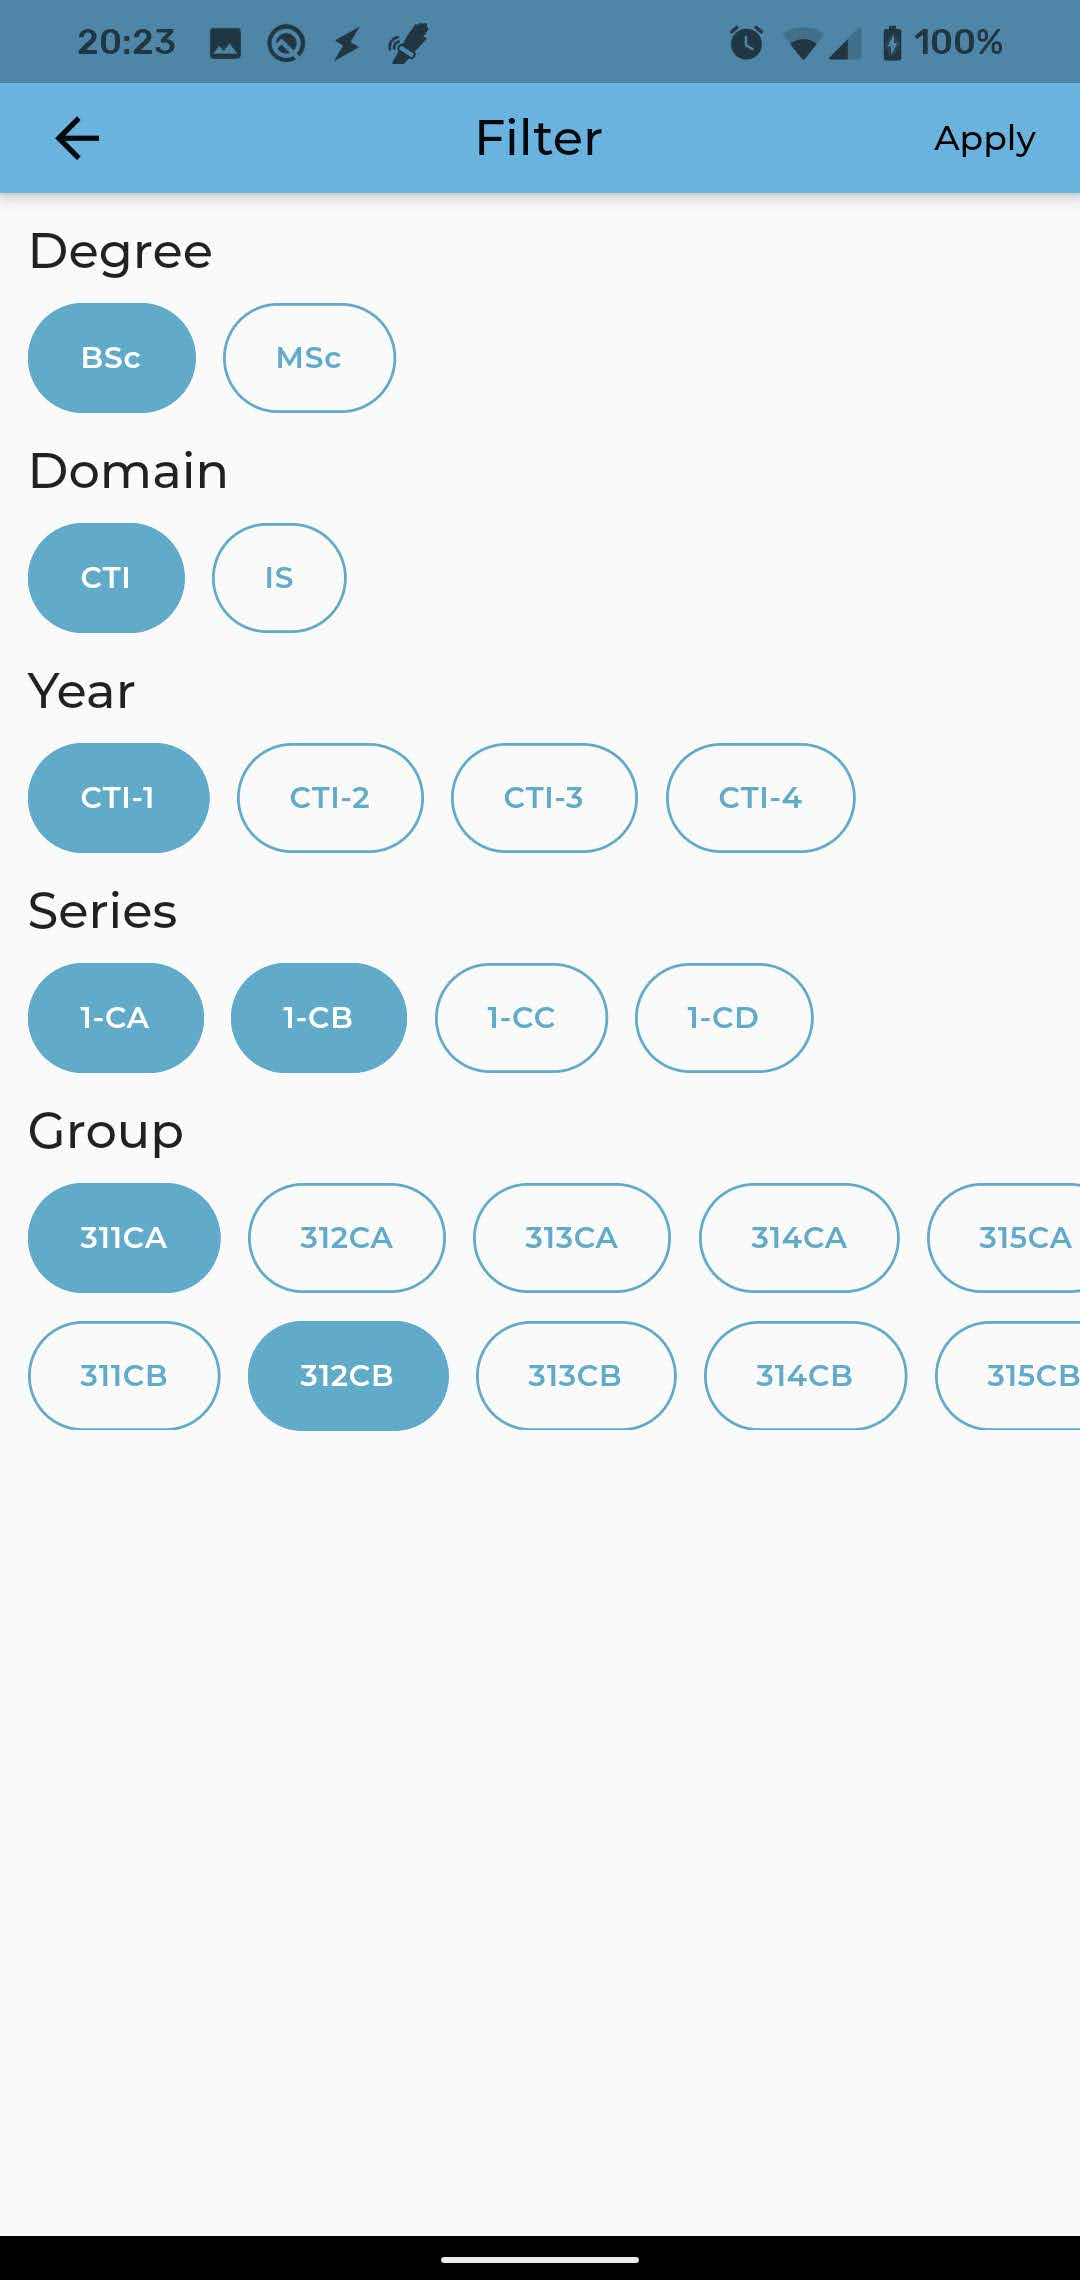
\includegraphics[width=\textwidth]{figures/app/flutter/filter.jpg}
        \caption{Filter page}
        \label{4:fig:filter}
    \end{minipage}
\end{figure}

The classes page (fig. \ref{5:tab:classes}) allows the user to view information about the specific class (fig. \ref{4:fig:class}) and even the lecturer (\ref{4:fig:lecturer}).

\begin{figure}[!ht]
    \centering
    \begin{minipage}[b]{0.26\textwidth}
        \captionsetup{justification=centering}
        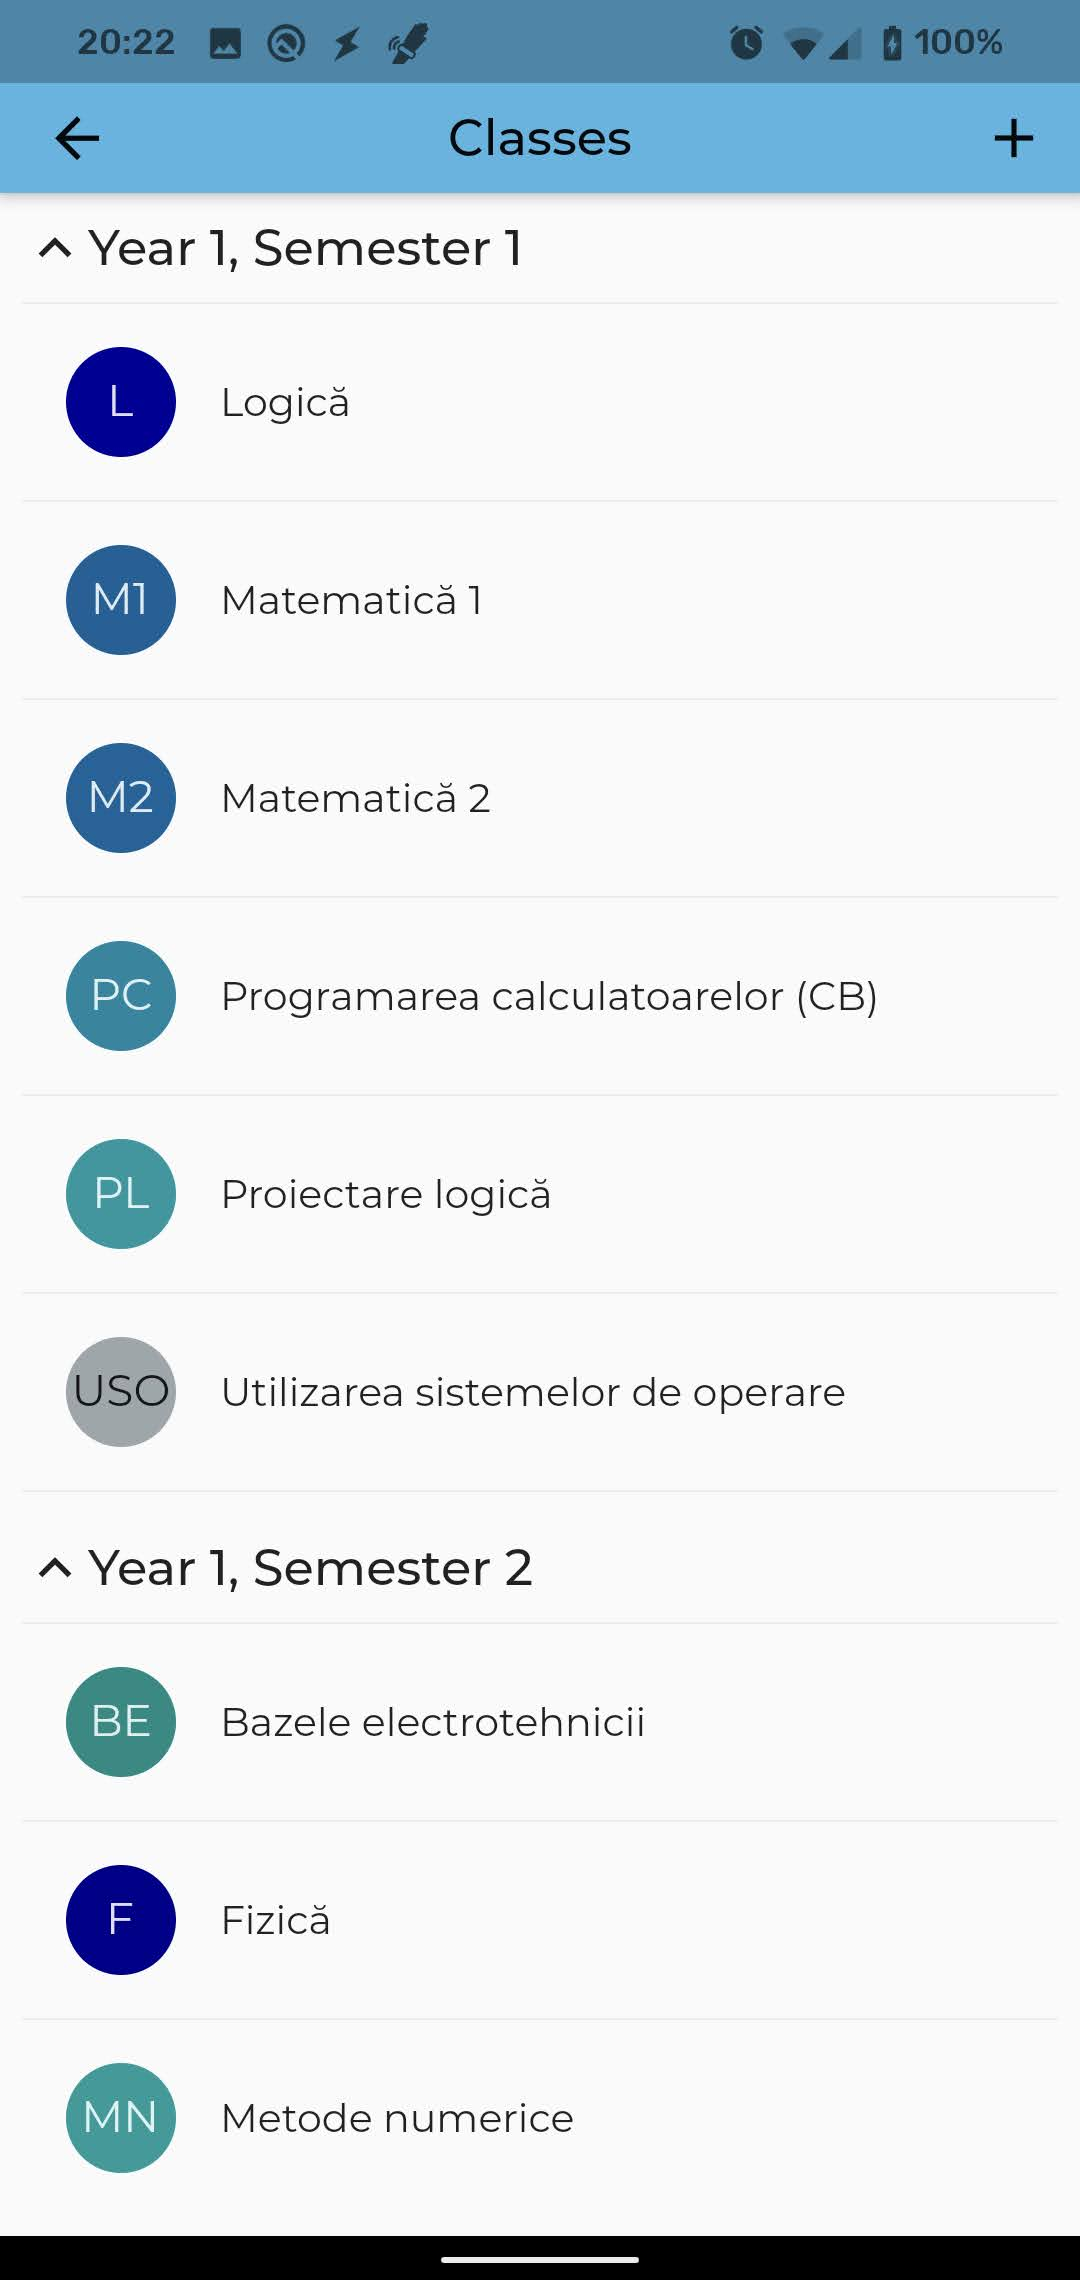
\includegraphics[width=\textwidth]{figures/app/flutter/classes.jpg}
        \caption{Classes page}
        \label{4:fig:classes}
    \end{minipage}
    \hfill
    \begin{minipage}[b]{0.26\textwidth}
        \captionsetup{justification=centering}
        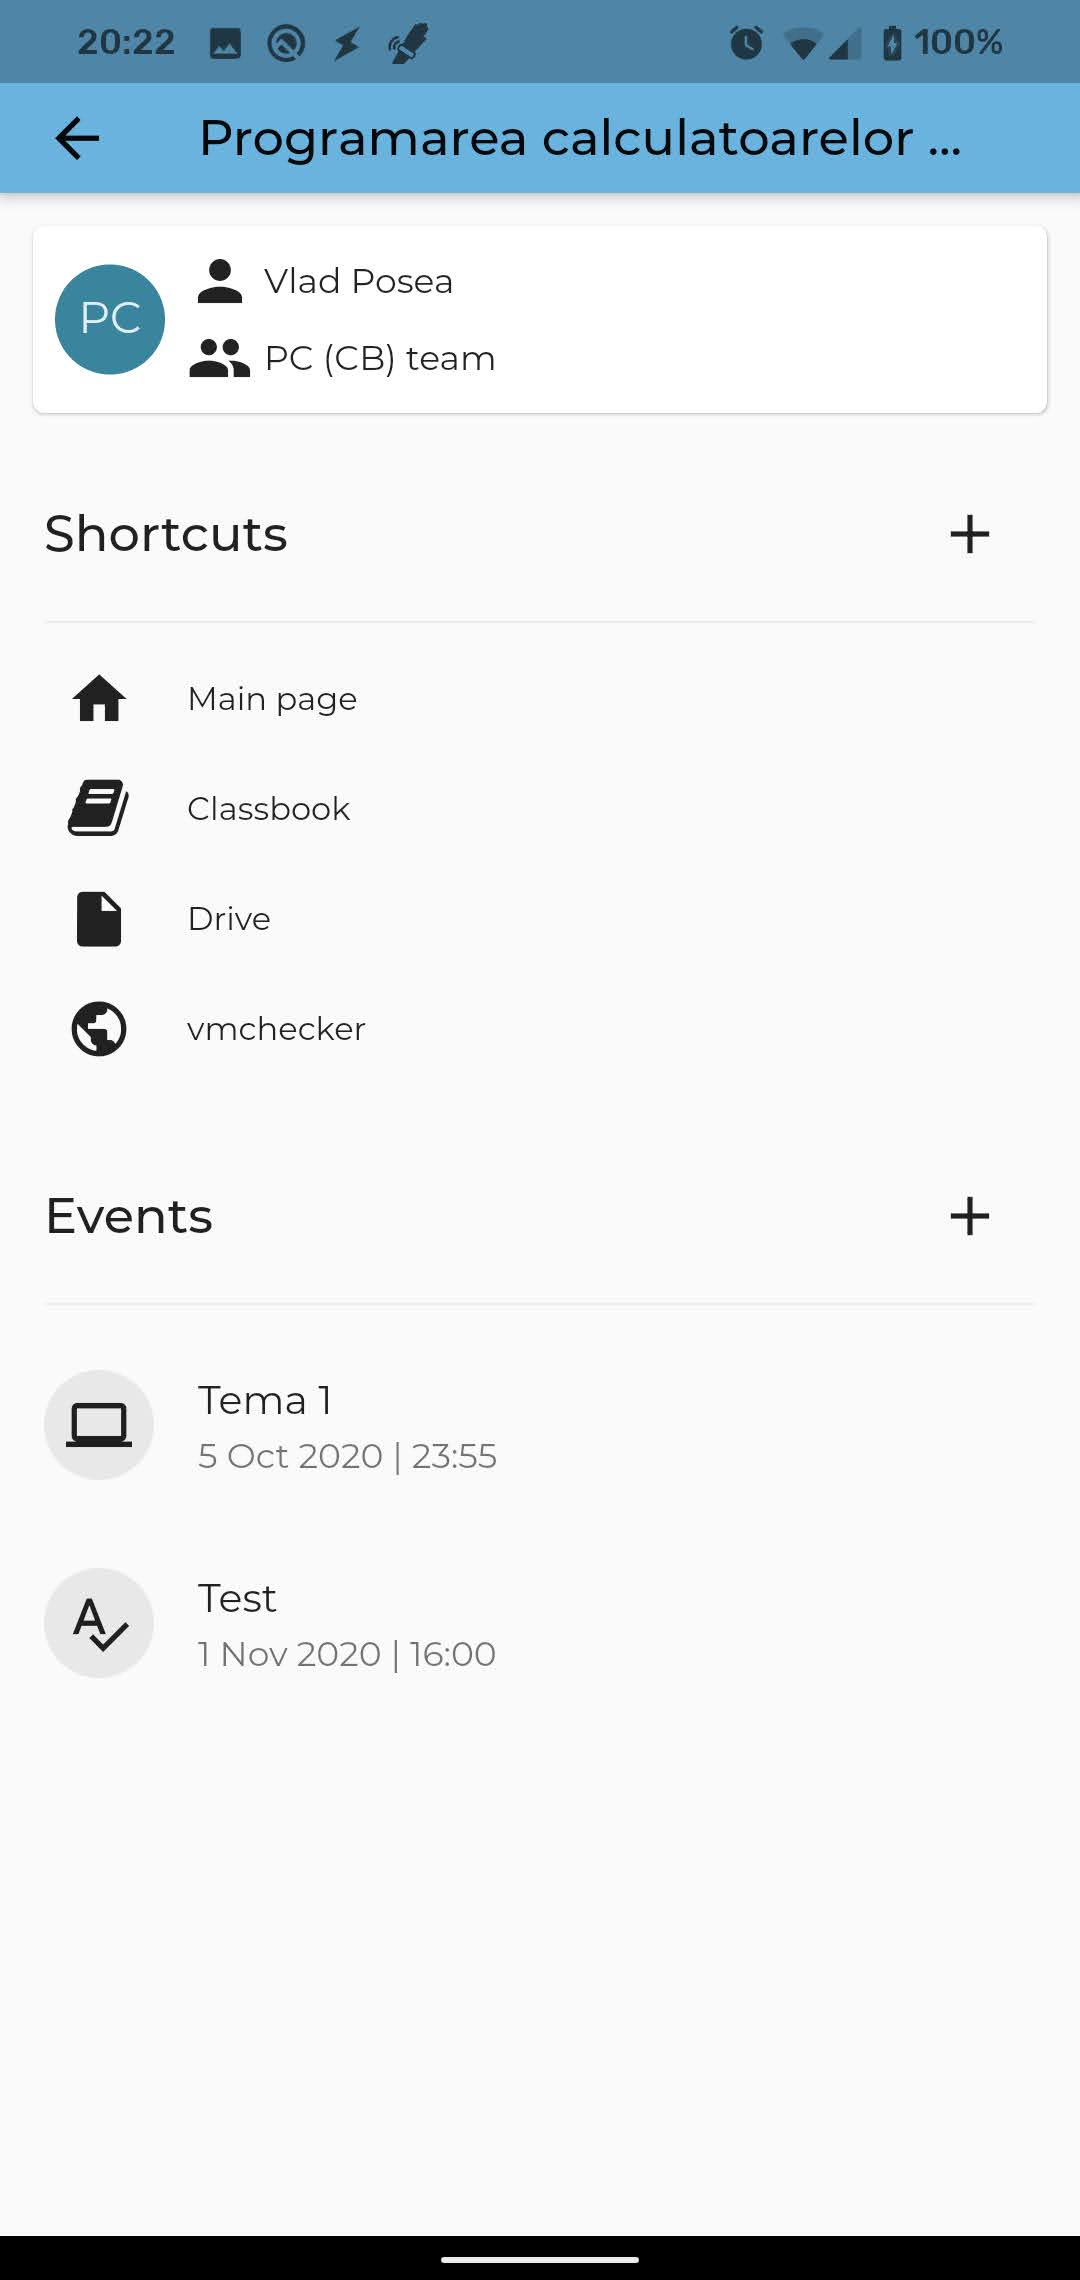
\includegraphics[width=\textwidth]{figures/app/flutter/class.jpg}
        \caption{Class information page}
        \label{4:fig:class}
    \end{minipage}
    \hfill
    \begin{minipage}[b]{0.26\textwidth}
        \captionsetup{justification=centering}
        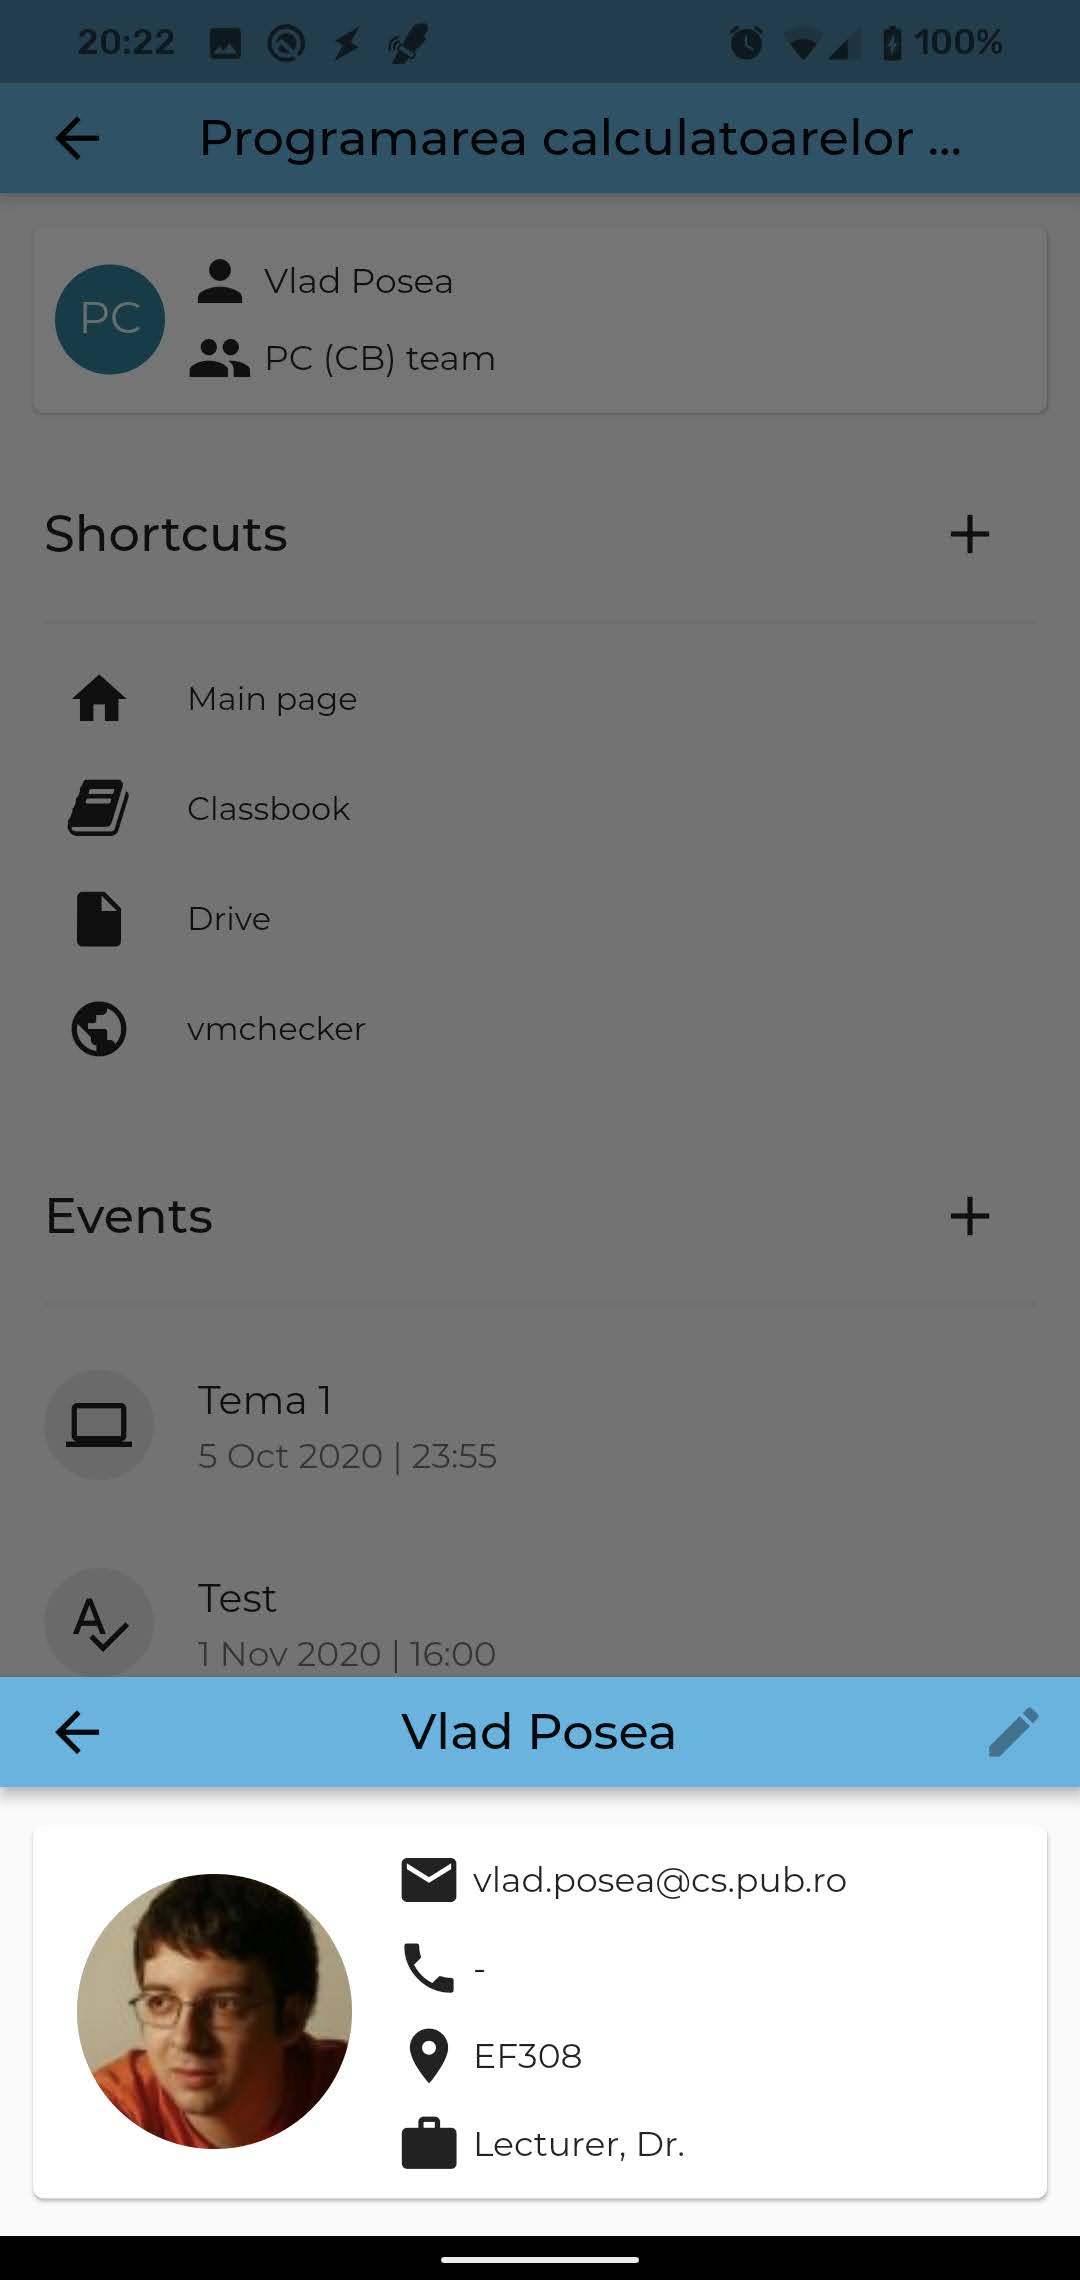
\includegraphics[width=\textwidth]{figures/app/flutter/lecturer.jpg}
        \caption{Lecturer information modal}
        \label{4:fig:lecturer}
    \end{minipage}
\end{figure}

\clearpage

The timetable page (fig. \ref{4:fig:timetable}) acts as a specialized calendar for university activities. Users can add and edit various events (fig. \ref{4:fig:edit_event}) that can be linked to a specific class, as well as view details about existing events (fig. \ref{4:fig:event}).

\begin{figure}[!ht]
    \centering
    \begin{minipage}[b]{0.26\textwidth}
        \captionsetup{justification=centering}
        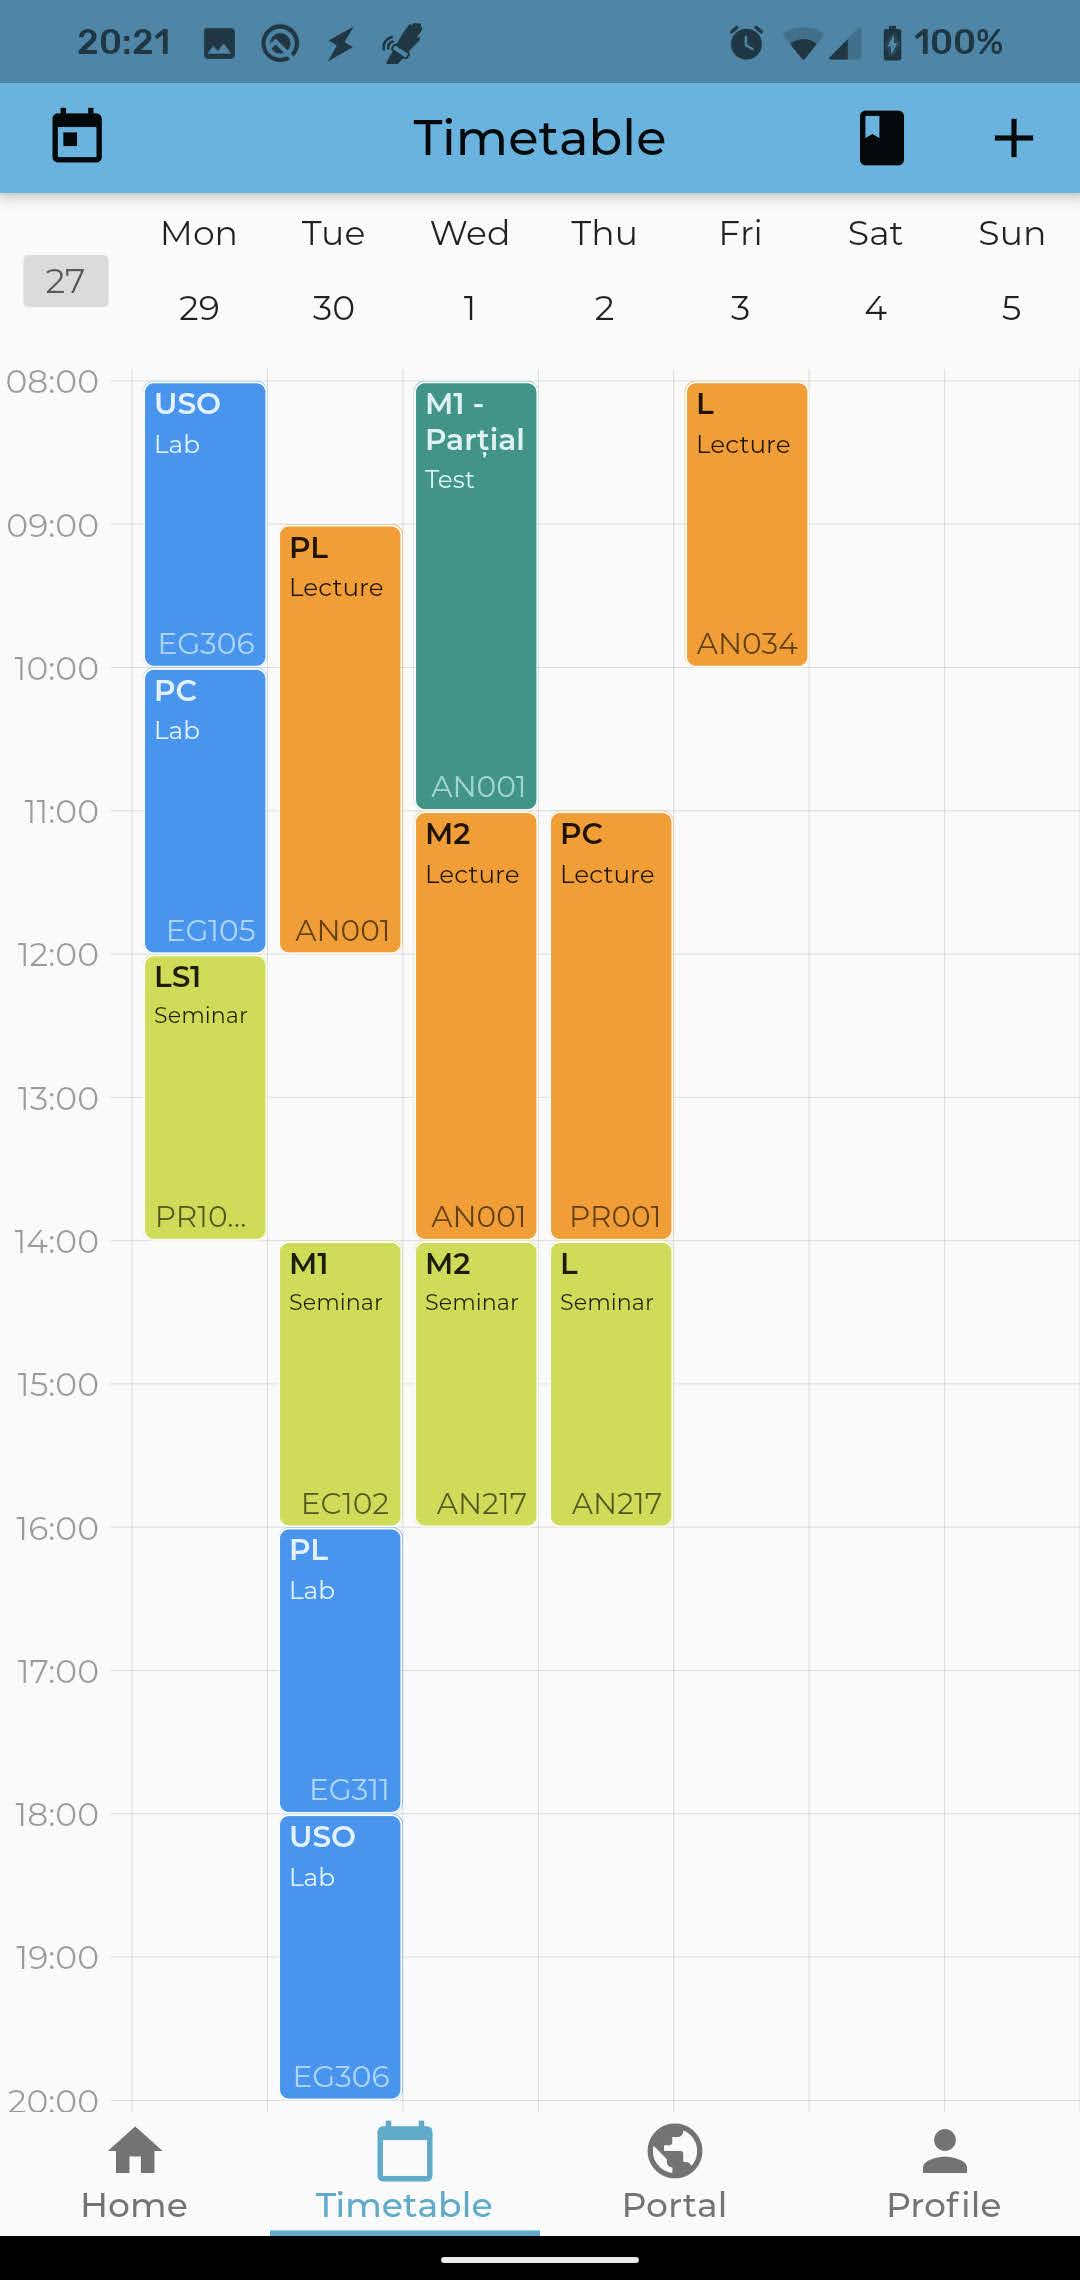
\includegraphics[width=\textwidth]{figures/app/flutter/timetable.jpg}
        \caption{Timetable page}
        \label{4:fig:timetable}
    \end{minipage}
    \hfill
    \begin{minipage}[b]{0.26\textwidth}
        \captionsetup{justification=centering}
        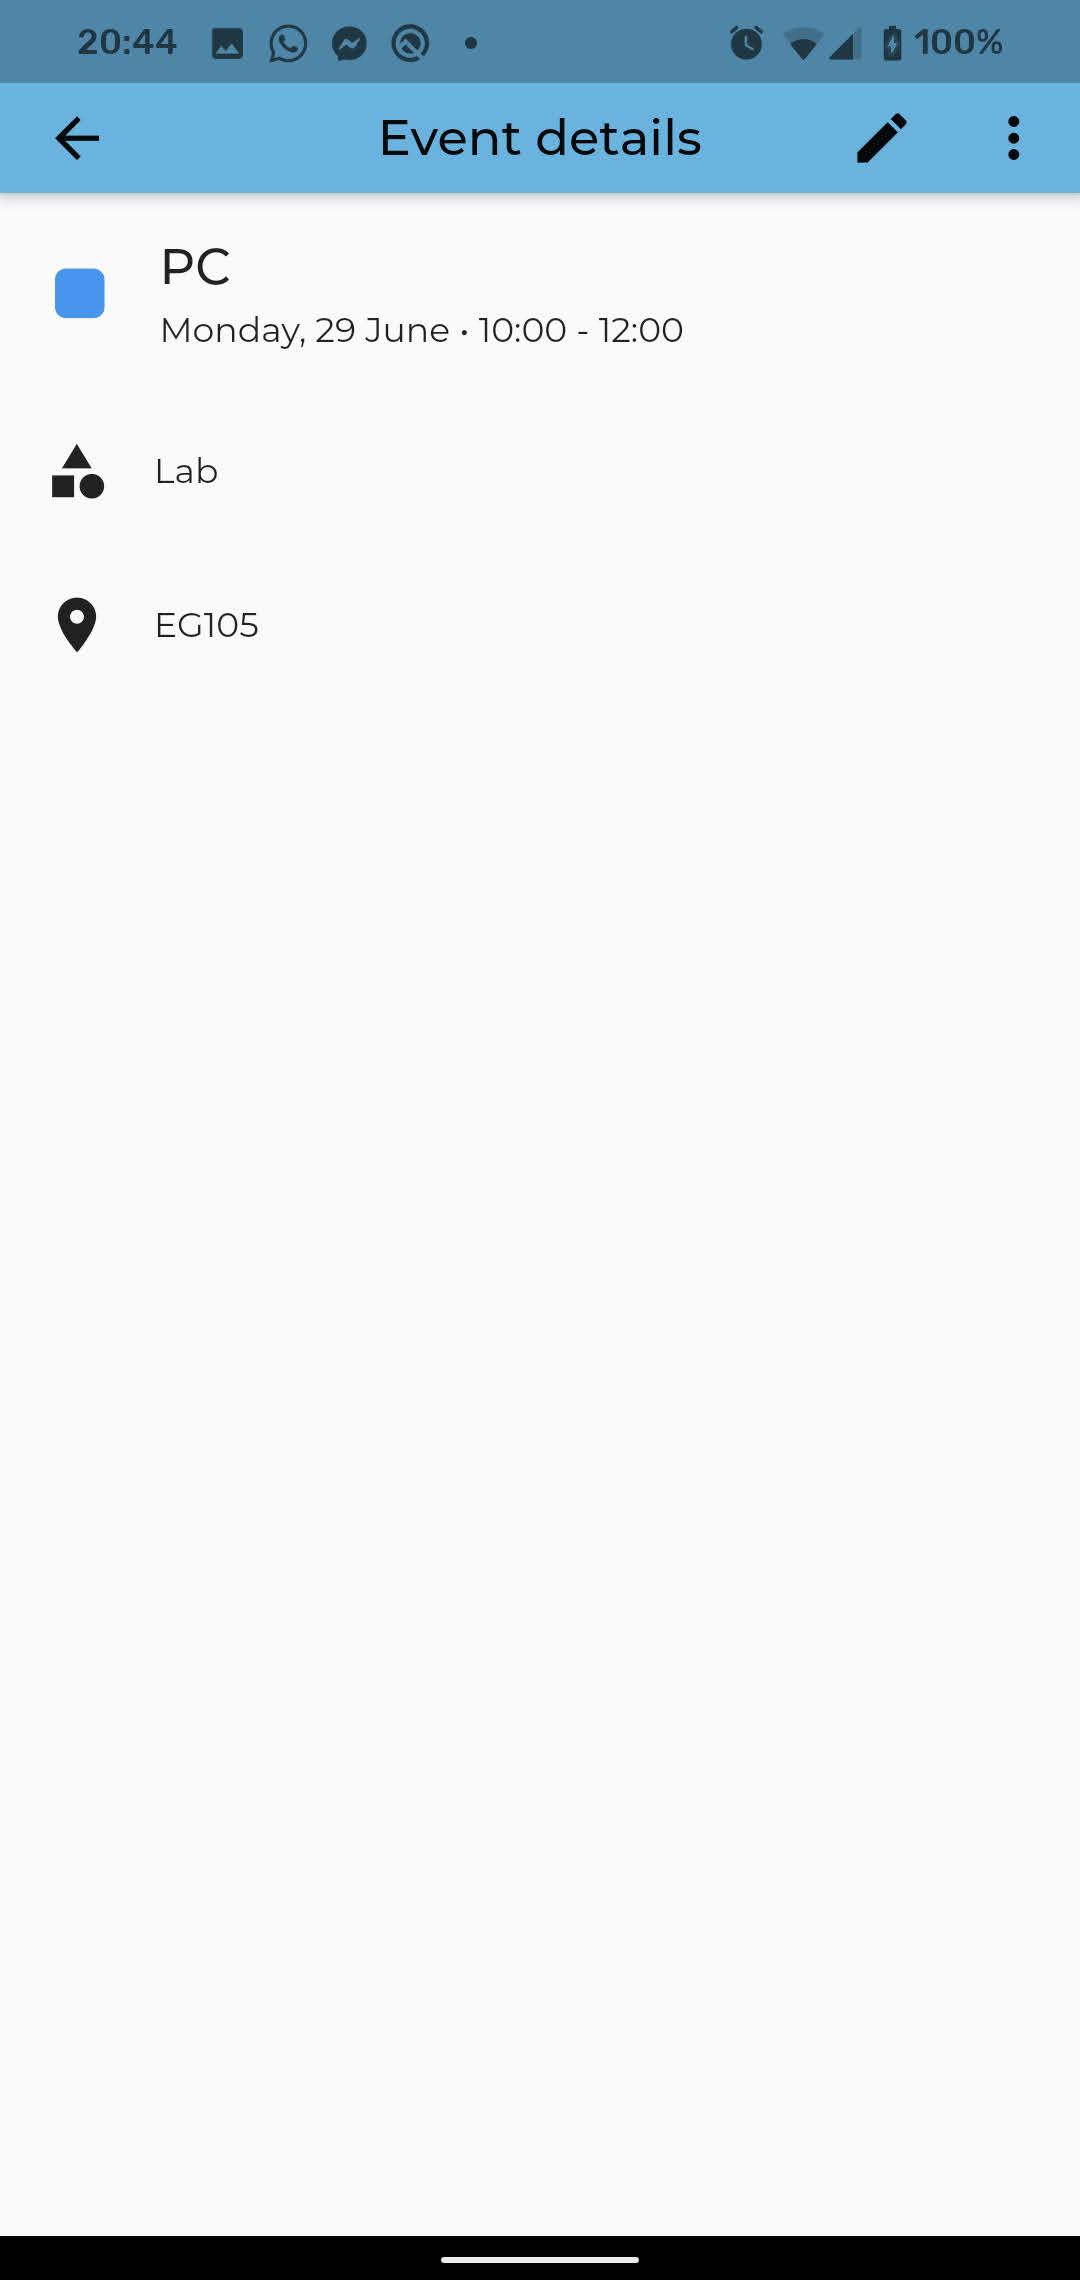
\includegraphics[width=\textwidth]{figures/app/flutter/event.jpg}
        \caption{Event information page}
        \label{4:fig:event}
    \end{minipage}
    \hfill
    \begin{minipage}[b]{0.26\textwidth}
        \captionsetup{justification=centering}
        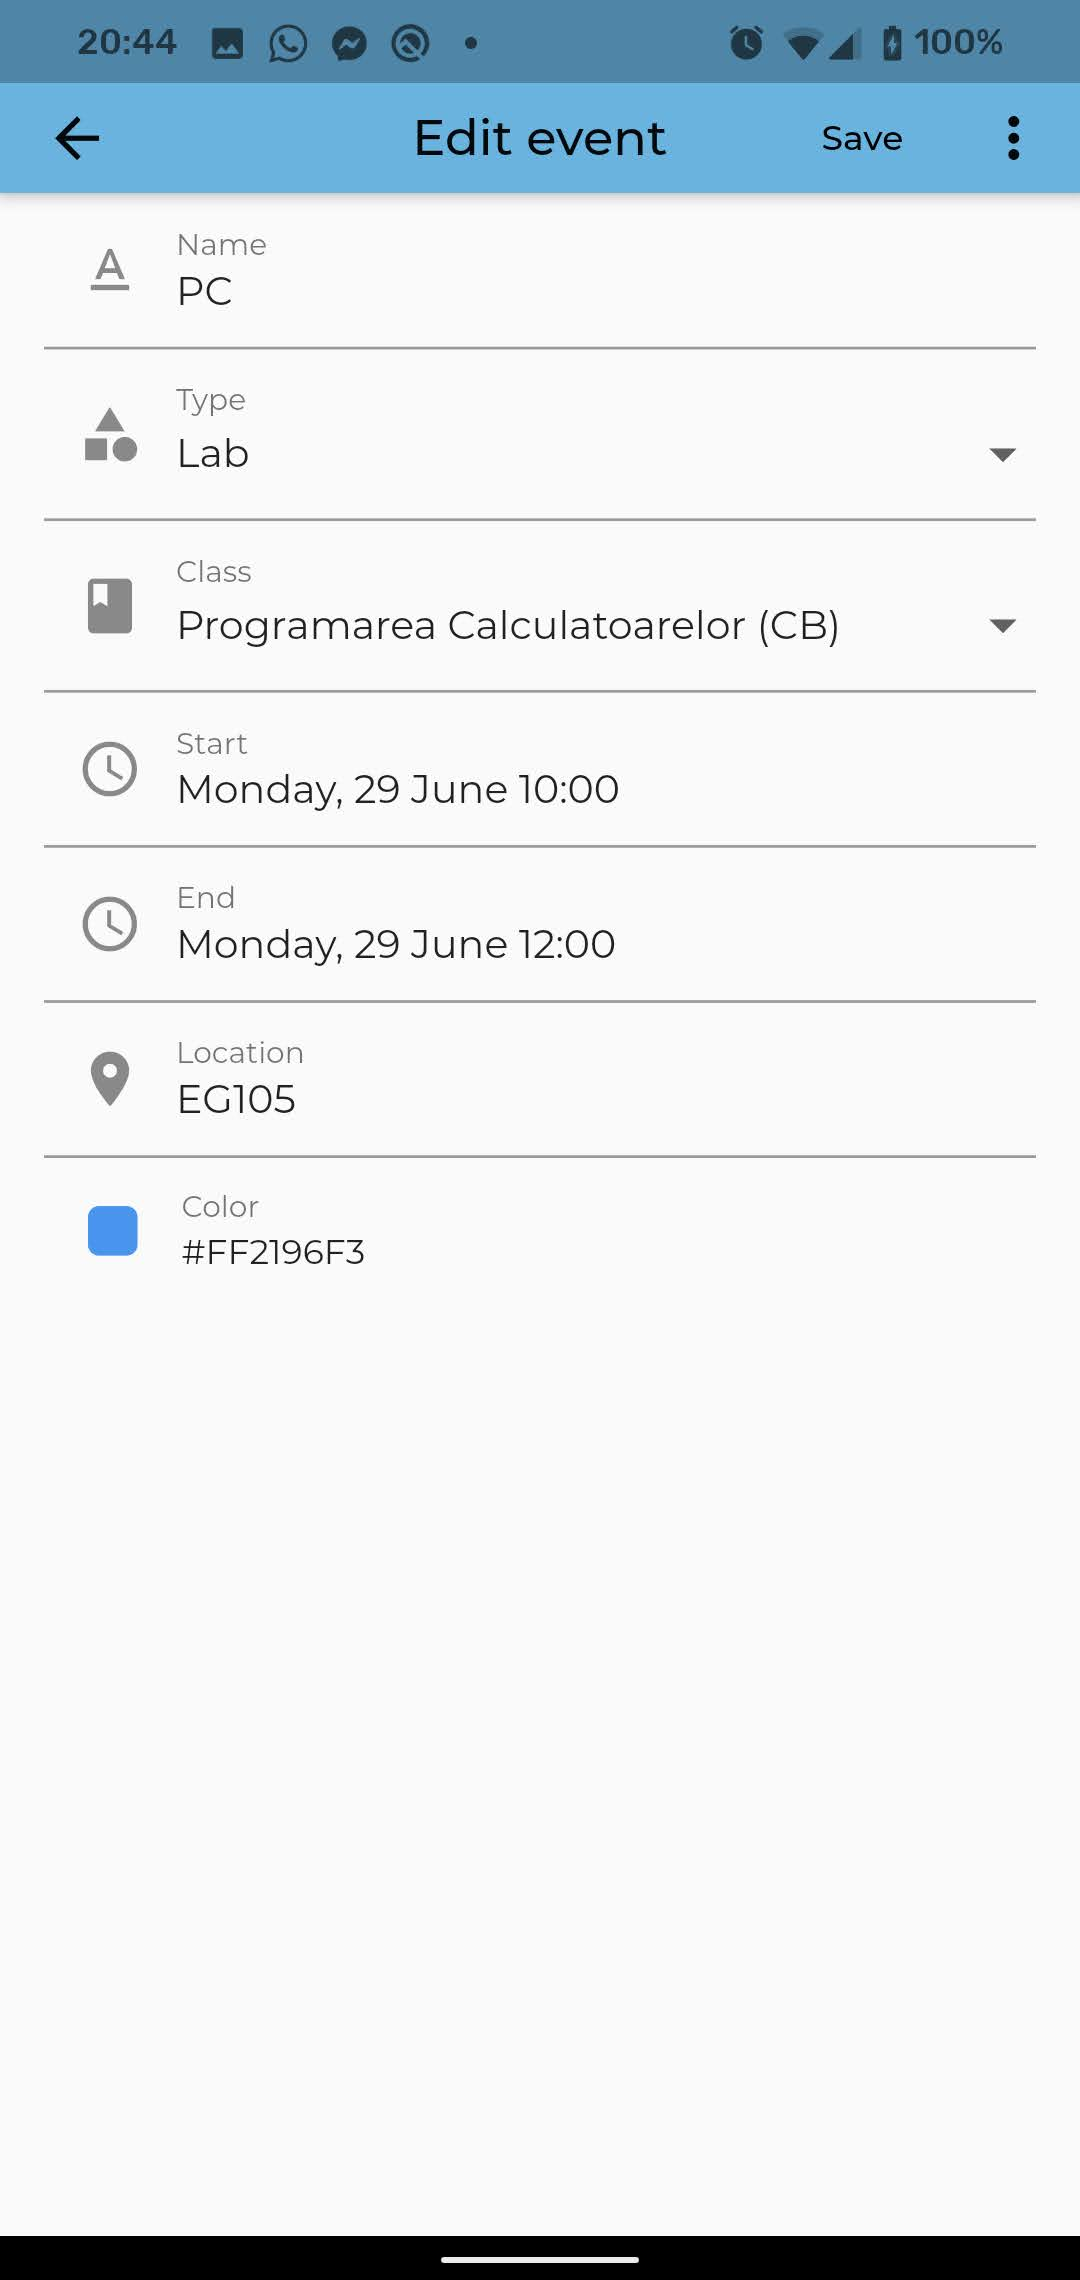
\includegraphics[width=\textwidth]{figures/app/flutter/edit_event.jpg}
        \caption{Edit event page}
        \label{4:fig:edit_event}
    \end{minipage}
\end{figure}